\documentclass[11pt,a4paper]{article}
\usepackage[margin=2.5cm]{geometry}
\usepackage[T1]{fontenc}
\IfFileExists{lmodern.sty}{\usepackage{lmodern}}{}
\usepackage{microtype,amsmath,amssymb,amsthm,booktabs,array,tabularx,xcolor}
\usepackage{enumitem}
\usepackage{graphicx}
\usepackage{tikz}
\usetikzlibrary{arrows.meta,positioning,calc}
\usepackage[authoryear,round]{natbib}
\setcitestyle{aysep={,},yysep={;}}
\usepackage{xurl}
\usepackage{hyperref}
\hypersetup{colorlinks=true,linkcolor=blue!45!black,citecolor=blue!45!black,urlcolor=blue!45!black}
\setlist{nosep,leftmargin=*}
\emergencystretch=2em

\newcommand{\softplus}{\operatorname{softplus}}
\newcommand{\topk}{\operatorname{top}_k}
\newcommand{\maybeincludegraphics}[2][]{%
  \IfFileExists{#2}{\includegraphics[#1]{#2}}{%
    \fbox{\parbox[c][3.2cm][c]{0.92\textwidth}{\centering
      \textit{Original figure file was not supplied}\\[5pt]
      \texttt{\detokenize{#2}}\\[3pt]
      \footnotesize Add the original figure next to this .tex to display it.}}}%
  }
\newcolumntype{L}{>{\raggedright\arraybackslash}X}
\newcolumntype{P}[1]{>{\raggedright\arraybackslash}p{#1}}
\newtheorem{proposition}{Proposition}

\title{\bfseries ENGRAMMER-DOPA: Novelty from failed identification in sparse neural representations\\[6pt]
\large\mdseries A signed-XOR mechanism for dopamine-like memory allocation}

\author{Jes\'us Marco de Lucas\\[2pt]
\small Instituto de F\'isica de Cantabria (IFCA), CSIC--Universidad de Cantabria, Santander, Spain\\
\small \texttt{jesus.marco@csic.es}}
\date{Preprint, 10 October 2026}

\begin{document}
\maketitle

\begin{abstract}
How can a neural circuit distinguish a new experience from one it already knows, and how can that distinction protect existing memories? We study these questions in a sparse signed-XOR autoencoder. A small set of latent neurons first reconstructs the current input. The difference between the input and its reconstruction identifies the input bits that the code has failed to explain. In this autoencoder the XOR output projects back to the latent neurons, where it instructs their plasticity. We point out that it also drives their activity. If the inhibition established by the first response is held while it does so, a well-explained input leaves the population sparse, whereas an unexplained one recruits additional neurons. We use the number of these extra active neurons as a signal of novelty.

We next test whether this signal can determine which neurons learn a new item. A dopamine-like pulse changes the competition for the final sparse code by favouring neurons with low previous use; an optional second action increases the learning rate. We distinguish three claims throughout: (H1) excess population activity can report novelty, (H2) novelty can guide memory allocation, and (H3) biological dopamine implements this link. The simulations test H1 and H2, not H3.

In sequential learning of 50 children's melodies, feedback makes even a frozen random latent layer an effective novelty detector: 98\% of learned contexts activate exactly 8 of 4,096 units, compared with a median of 27 units for held-out contexts (AUC 0.996). Without feedback the AUC is 0.50. In a plastic autoencoder, retention without modulation is 0.36. Novelty-timed allocation raises retention to 0.92 and free recall to 0.87; the same pulses at shuffled times give 0.64 and 0.49. A count of unexplained input bits can also detect novelty and, at matched pulse rates, guide allocation equally well. The difference is that the learned latent signal tolerates small perturbations of familiar contexts and is less sensitive to presentation noise. In a synthetic world, the full novelty-controlled intervention reduces collisions between similar memories to 2\%, compared with 30\% without modulation and 20\% at shuffled times. In class-incremental MNIST, novelty timing helps when older classes recur or are replayed, but not when they never return. These results support a specific computational role for a global modulatory signal: deciding \emph{which neurons} store an experience, rather than simply increasing learning everywhere.
\end{abstract}

\noindent\textbf{Keywords:} dopamine; novelty; sparse coding; autoencoder; feedback inhibition; homeostatic plasticity; memory allocation; continual learning; signed-XOR.

%======================================================================
\section{Introduction}

\subsection*{The problem: learning without overwriting}
An animal encounters both familiar and unfamiliar experiences. A familiar experience should normally activate an existing memory. An unfamiliar one should be stored, ideally without destroying a similar memory that is already there. This raises two different questions: \emph{How does the circuit identify that the current input has not been learned?} And \emph{how does that decision change the neurons that will learn it?}

Dopamine is relevant to the second question. Novel experiences can engage dopaminergic systems and promote the persistence of memories \citep{lisman2005,duszkiewicz2019,moncada2007,takeuchi2016}. Dopamine can make synaptic changes persist within restricted time windows \citep{shindou2019,yagishita2014} and can alter neuronal excitability \citep{durstewitz2008,kutter2026,naude2024}. None of these observations, however, identifies a single computation by which a circuit decides that its \emph{present input} is novel.

Novelty is often estimated from a separate record of familiarity, such as visitation counts or learned familiarity weights \citep{kakade2002,bogacz2003,dasgupta2018}. Another possibility is to use \emph{surprise}: the failure to predict the next event \citep{modirshanechi2022}. But novelty and surprise are different \citep{xu2021}. A sudden switch between two familiar stimuli can be surprising without introducing anything new; conversely, the first presentation of a new stimulus is novel even when there is no temporal prediction to violate. We seek a signal for identification failure, not transition surprise.

\subsection*{The proposed mechanism}
The starting point is an autoencoder that stores each input using a sparse set of latent neurons. Its code attempts to reconstruct the current input. A signed-XOR comparison identifies both the input bits that were missed and the bits that were incorrectly reconstructed \citep{pena2026loss}. In the signed-XOR autoencoder these channels project back to the latent neurons; this is how the code learns. Our proposal concerns what this projection does to latent \emph{activity}, not only to plasticity: with inhibition held at the level set by the first response, the missed bits recruit latent neurons beyond the code, and their number can be read as novelty. The mechanism can be understood as a sequence of five operations:
\begin{enumerate}[label=\arabic*.]
\item The input activates a provisional set of $k$ neurons. This initial response also establishes an inhibitory level.
\item These $k$ neurons reconstruct the input. A signed-XOR comparison identifies which input bits were not reconstructed.
\item The XOR output reaches the latent population, as it does for learning. The missed bits excite latent neurons, and the inhibition established in step 1 does not rise. An unfamiliar input can therefore recruit neurons beyond the original $k$.
\item The number of \emph{additional} active neurons provides the novelty signal.
\item If that signal exceeds a threshold, a dopamine-like pulse biases the competition for the final $k$-neuron code towards neurons that have been used less often. Learning then updates this final code.
\end{enumerate}
A familiar input that is reconstructed correctly produces no returning error and no excess activity. Importantly, the mechanism distinguishes the \emph{population response that detects novelty} from the \emph{sparse code that stores the input}. These are not the same set of active neurons.

The allocation step is motivated by two established ideas. Intrinsic excitability can decrease through homeostatic adaptation after repeated activity \citep{desai1999,turrigiano2008}. Separately, neurons with greater excitability are more likely to be recruited into a memory trace \citep{josselyn2018,yiu2014}. We hypothesise that a dopamine-like signal temporarily amplifies the resulting differences in excitability, favouring little-used neurons when an input is not identified. The precise dopaminergic dependence is a proposed biological mechanism, not a measured property of these simulations.

\subsection*{Claims and experimental strategy}
We separate the argument into three claims. \textbf{H1 (detection):} excess latent activity can identify inputs that the network has not learned. \textbf{H2 (allocation):} the detected novelty can guide competition for coding neurons and thereby reduce interference. \textbf{H3 (biological interpretation):} dopamine provides this modulatory link in neural tissue. We test H1 and H2 computationally. H3 generates experimental predictions but remains untested.

What is new is therefore not the projection of the error to the latent layer, which the autoencoder already has, but three things: holding the initial inhibition while the projection acts, reading the resulting excess as novelty, and using it to allocate memory. Versions up to 0.7 of this work computed novelty from the feedforward response alone and so ignored the effect of this projection on activity. Section~\ref{sec:model} gives the mechanism and its learning rules, all based on signed-XOR updates \citep{pena2026motif,pena2026loss}. We then test three deliberately different situations. A small synthetic world lets us distinguish new stimuli from unexpected \emph{transitions} between familiar stimuli (Section~\ref{sec:toy}). Class-incremental MNIST tests whether allocation reduces interference among related images, with and without recurrence of earlier classes (Section~\ref{sec:mnist}). Finally, sequential learning of 50 children's melodies \citep{pena2026songs} provides the clearest test of detection, memory retention, and free recall, and allows a direct comparison with the simpler count of unexplained input bits (Section~\ref{sec:songs}). Section~\ref{sec:predictions} describes possible biological tests; Section~\ref{sec:discussion} discusses limitations. A negative earlier experiment on transition surprise is preserved in Appendix~\ref{app:surprise}.

\section{Model}\label{sec:model}

\subsection{Overview and notation}
The network has $D$ binary input lines and $N$ latent neurons. Only $k$ latent neurons are selected to store any one input, with $k\ll N$. There are two stages. The first produces a \emph{provisional} code and measures whether its reconstruction explains the input. The second, after an optional dopamine-like pulse, selects the \emph{final} code on which learning acts. Keeping these two stages separate is essential: otherwise the modulation that changes the code could also change the novelty signal used to trigger it.

For reference, the principal quantities are summarised below. The input comparison and the latent comparison both use signed-XOR channels, but at different layers.
\begin{center}
\small
\begin{tabularx}{\textwidth}{@{}P{2.5cm}L@{}}
\toprule
Symbol & Meaning \\
\midrule
$x_t$ & Current binary input (dimension $D$) \\
$a_t$ & Initial, feedforward drive to the $N$ latent units \\
$c^{(0)}_t$ & Provisional code: the $k$ strongest feedforward units \\
$\hat x_t$ & Reconstruction obtained from the provisional code \\
$C^+_t, C^-_t$ & Input bits missed by, and falsely added by, the reconstruction \\
$f_t$ & Feedback drive produced by the missed input bits \\
$z_t$ & Units active after feedback, against the original inhibitory threshold \\
$\nu_t$ & Number of active units outside the provisional code, divided by $k$ \\
$D_t$ & Binary dopamine-like pulse, triggered by novelty \\
$c_t$ & Final $k$-neuron code selected for learning \\
\bottomrule
\end{tabularx}
\end{center}

\subsection{Stage 1: form a provisional code and reconstruct the input}
For input $x_t\in\{0,1\}^D$, each neuron $j$ receives a feedforward cosine-similarity drive through non-negative weights $V\in[0,1]^{D\times N}$:
\[
a_{j,t}=\frac{V_{\cdot j}^{\top}x_t}{\|V_{\cdot j}\|\,\|x_t\|}.
\]
The $k$ strongest neurons define $c^{(0)}_t=\topk(a_t)$. This fixed code size is the network's sparsity set-point \citep{marco2024worms}. It is not yet the code that will be learned.

The provisional code reconstructs each input bit through decoder weights $U$:
\[
\hat x_{i,t}=\mathbf 1\!\left[\sum_{j\in c^{(0)}_t}U_{ij}\ge k\theta\right],\qquad\theta=\tfrac12.
\]
In a \emph{tied} autoencoder, $U=V$. In the frozen-encoder experiments, the random encoder $V$ stays fixed while a separate decoder $U$ learns. Comparing $\hat x_t$ with $x_t$ gives the two signed-XOR channels \citep{pena2026loss}:
\[
C^+_{i,t}=x_{i,t}(1-\hat x_{i,t}),\qquad
C^-_{i,t}=(1-x_{i,t})\hat x_{i,t}.
\]
Thus $C^+$ identifies a bit that is present in the input but absent from the reconstruction (\emph{missed evidence}); $C^-$ identifies a bit reconstructed despite being absent from the input (\emph{false evidence}). Both reach the latent neurons and guide their learning. Only $C^+$ is assumed to excite them (Stage~2).

\subsection{Stage 2: the XOR output drives the latent population while inhibition is held fixed}
The XOR output that instructs latent plasticity also reaches latent activity. In the model, the missed input bits act on the latent population through the same afferent weights as the input. For neuron $j$, the total drive is
\begin{equation}
 a'_{j,t}=a_{j,t}+\lambda\,f_{j,t},\qquad f_{j,t}=\frac{V_{\cdot j}^{\top}C^+_t}{\|V_{\cdot j}\|\,\|x_t\|},
 \label{eq:feedback}
\end{equation}
where $\lambda\ge0$ controls feedback strength. A unit responds strongly to the returning error if its weights match the bits that the provisional code failed to reconstruct. Only $C^+$ drives activity. In the signed-XOR motif, $C^-$ is carried by an inhibitory aggregator \citep{pena2026motif}; if its projection to the latent layer has the same sign, $C^-$ can only lower latent activity and cannot recruit units, and the asymmetry follows from Dale's principle rather than from a modelling choice. Whether the projection in a given circuit has this sign structure is an empirical question.

\paragraph{Why inhibition must be held fixed.}
The initial feedforward response establishes the inhibition \emph{before} the error returns. We consider two choices. An earlier version used $T_t=\gamma\max_j a_{j,t}$, with $\gamma<1$. The main experiments instead use the drive of the $k$-th strongest feedforward unit, $T_t=a_{(k),t}$. The population response after feedback is
\begin{equation}
 z_{j,t}=\mathbf 1\big[a'_{j,t}\ge T_t\big].
 \label{eq:inhib}
\end{equation}
With $T_t=a_{(k),t}$ and no returning error, exactly the $k$ provisional neurons are active (apart from ties). A correctly reconstructed input still activates only these $k$ neurons. A new input can activate additional neurons because feedback raises their drive without raising $T_t$.

This fixed-threshold assumption is substantive, and it has two parts. First, setting the inhibitory level at the $k$-th strongest initial unit is an idealised operation that makes the initial response sparse by construction; a biological circuit would have to approximate it. Second, the level must not rise when the error returns. If inhibition were recomputed after feedback so as to force exactly $k$ winners, the additional activity would disappear. With $T_t=\gamma\max a$, by contrast, many random neurons can cross the threshold even before feedback: in the frozen melody experiment 93 of 4{,}096 units are active for learned and new inputs alike. We therefore use inhibition at the $k$-th winner throughout the current experiments, retaining the other rule as a control and as the feedforward special case of version 0.7. Whether biological inhibition has the required timing is a central prediction of the proposal (P4).

\subsection{Stage 3: measure novelty from the excess response}\label{sec:novelty}
Let $z_{j,t}$ indicate whether a neuron is active \emph{after} feedback. We count neurons that have become active but are not members of the provisional $k$-neuron code:
\begin{equation}
 \nu_t=\frac1k\sum_j z_{j,t}\big(1-c^{(0)}_{j,t}\big).
 \label{eq:novelty}
\end{equation}
The division by $k$ expresses the excess in units of the nominal code size. Thus $\nu_t=0$ means no extra active units, and $\nu_t=1$ means $k$ additional active units. This is a population-level measure of \emph{failure to identify the current input}; it is not a measure of the surprise of the preceding transition. We use \emph{identification} rather than recognition in the autoencoder sense, which would require exact reconstruction: an input is identified when its provisional code explains all of its present bits, even if the reconstruction adds bits that are absent (Proposition~\ref{prop:ident}).

\begin{proposition}[Identification criterion]\label{prop:ident}
Let inhibition be set at the $k$-th winner, $T_t=a_{(k),t}$. Then (i) every unit of $c^{(0)}_t$ is active, so that $|z_t|=k(1+\nu_t)$; (ii) a unit $j\notin c^{(0)}_t$ is active if and only if $\lambda f_{j,t}\ge a_{(k),t}-a_{j,t}$; (iii) if the provisional code reconstructs the input, $C^+_t=0$, then $\nu_t=0$, and conversely $\nu_t>0$ implies $C^+_t\ne0$; (iv) $\nu_t$ is unchanged if all drives $a_t$ and $f_t$ are multiplied by the same positive factor, as by a uniform change of gain. With $\lambda=0$ and $T_t=\gamma\max_ja_{j,t}$, $k\nu_t=\big|\{j>k:\ a_{(j),t}\ge\gamma a_{(1),t}\}\big|$, the contrast criterion of version 0.7.
\end{proposition}

The proposition explains the detection mechanism precisely. A reconstruction with no missed input bits necessarily produces no excess. If there is excess activity, some input bits must have been missed. The reverse implication does \emph{not} hold: a small mismatch may fail to drive any additional neuron above threshold. The feedback gain $\lambda$ determines how tolerant the system is to such mismatches. Small $\lambda$ makes it easier to identify a noisy version of a learned item; large $\lambda$ makes the detector more sensitive to missed bits. The measure is also unchanged by a uniform multiplicative rescaling of the drives.

There are two important limitations. First, only $C^+$ recruits units, so an input that is \emph{missing} part of a stored pattern may be identified as familiar if the reconstruction merely adds the absent bits ($C^-\ne0$). Letting $C^-$ excite latent units as well, a non-physiological variant if $C^-$ is inhibitory, improves detection of such deletions but can destroy exact sparsity on learned inputs (Section~\ref{sec:songs}). Second, $\nu_t$ is not simply the magnitude of reconstruction error. A few missed bits may bring many near-threshold neurons above inhibition; many missed bits may bring none if their projections are weak. The learned geometry of the encoder therefore matters.

\begin{proposition}[Novelty is the depression channel of a population signed-XOR]\label{prop:sxor}
Apply the signed-XOR operator \citep{pena2026motif,pena2026loss} unit by unit with target $q_j=c^{(0)}_j$ and output $o_j=z_j$. The depression channel $C^-_j=(1-q_j)o_j$ marks the active units outside the provisional code, and $\sum_jC^-_j=k\nu_t$. The potentiation channel $C^+_j=q_j(1-o_j)$ marks code units below the inhibitory threshold; it is zero when inhibition is set at the $k$-th winner, and with $T_t=\gamma\max a$ it is non-zero only when fewer than $k$ units are active.
\end{proposition}

There are therefore \emph{two separate signed-XOR comparisons}. The first compares $x_t$ and $\hat x_t$ at the input layer and sends missed bits back to the latent layer. The second compares the provisional code with the post-feedback population response. Its summed depression channel equals the novelty signal. This identity does not establish a biological implementation, but it shows how the novelty readout could use the same local comparison motif as the learning rule \citep{pena2026motif}. Neither a stored familiarity counter nor a predictor of future states is required.

\subsection{Stage 4: learn through signed-XOR corrections}\label{sec:learning}
Only the \emph{final} code, defined below, receives the ordinary learning updates. Every update has the signed-XOR form $x_{ji}=y_i(C^+_j-C^-_j)$, multiplied by a learning rate and a non-negative plasticity gain $G_t$. The target determines what each connection learns:
\begin{itemize}
\item \textbf{Autoencoder reconstruction.} Using the final code $c_t$, the reconstructed input is $\hat x_{i,t}=\mathbf 1[\sum_{j\in c_t}U_{ij}\ge k/2]$. With the input as target, the decoder update is $\Delta U_{ij}=\eta\,G_t\,c_{j,t}(x_{i,t}-\hat x_{i,t})=\eta\,G_t\,c_{j,t}(C^+_{i,t}-C^-_{i,t})$ \citep{pena2026loss}. With tied weights $U=V$, the encoder changes as well; when the encoder is frozen, only $U$ changes.
\item \textbf{Optional depression of excess neurons.} A further signed-XOR depression channel can act on active units not included in the \emph{final} code: $C^-_{j,\rm learn}=(1-c_{j,t})z_{j,t}$, giving $\Delta V_{ij}=-\eta\,G_t\,c^-\,C^-_{j,\rm learn}\,x_{i,t}$. This differs from the novelty readout $C^-_{j,\rm nov}=(1-c^{(0)}_{j,t})z_{j,t}$: allocation can change the final code, so their sums need not agree. \textbf{This optional channel is disabled in all current experiments} ($c^-=0$). After feedback, hundreds of excess neurons can be active; depressing all their inputs caused learning collapse. With $c^-=0.5$ in MNIST, accuracy stayed below 0.3 in all streams.
\item \textbf{Predictor or output readout.} In the synthetic world, $W$ predicts the next latent code, with $\hat c_t=\mathbf 1[Wc_{t-1}>\vartheta]$ and $\Delta W=\eta_W G_t(c_t-\hat c_t)c_{t-1}^{\top}$. In MNIST, the label readout learns $\Delta R_{lj}=\eta_y G_t c_{j,t}(y_{l,t}-\hat y_{l,t})$, where $\hat y_{l,t}=\mathbf 1[\sum_{j\in c_t}R_{lj}\ge k/2]$. For melodies, an analogous readout predicts the next bar's pitch and onset, selecting the value with the strongest output drive (Section~\ref{sec:songs}).
\end{itemize}
Weights are clipped to their specified ranges. The modulatory pulse changes the competition for neurons and potentially the \emph{size} of the update; it never determines the sign of a signed-XOR correction.

\subsection{Stage 5: let novelty control memory allocation}\label{sec:dopamine}
A binary dopamine-like pulse is triggered when the excess crosses a threshold:
\[
D_t=\mathbf 1[\nu_t>\nu_{\rm th}].
\]
For example, $\nu_{\rm th}=1$ requires more than $k$ extra active neurons. The pulse can act in two ways, which are kept separate in our controls.

\paragraph{Allocation through homeostatic excitability.}
Neuron $j$ has an intrinsic excitability $e_{j,t}=1-\min(u_{j,t}/n_0,1)$, where $u_{j,t}$ counts how frequently the neuron has participated in final codes. The count decays slowly where specified. This gives highly used neurons lower intrinsic excitability, as suggested by homeostatic intrinsic plasticity \citep{desai1999,turrigiano2008}. During a pulse, the code is selected using the extra excitability:
\begin{equation}
 c_t=\topk\big(a_t+\kappa\,D_t\,e_t\big).
 \label{eq:alloc}
\end{equation}
When there is no pulse, $D_t=0$ and $c_t=c^{(0)}_t$. During a pulse, less-used neurons may displace highly used neurons, providing space for a new representation.

\begin{proposition}[Exciting the uncommitted is suppressing the committed]\label{prop:equiv}
With $m_{j,t}=\min(u_{j,t}/n_0,1)$, the code (\ref{eq:alloc}) equals $\topk(a_t-\kappa D_tm_t)$.
\end{proposition}

The identity follows because the two scoring rules differ by the same constant for every neuron (Appendix~\ref{app:proofs}). Dopamine therefore need not \emph{directly inhibit} used neurons. It would suffice to amplify intrinsic excitability so that the most excitable neurons have a competitive advantage, in line with engram-allocation studies \citep{josselyn2018,yiu2014}. The use-dependent excitability itself changes slowly, on the scale of hours or days \citep{desai1999}. The hypothesis is that dopamine transiently exploits these pre-existing differences. Its predicted quantitative selectivity remains untested (P5).

\paragraph{Timing.}
The order of events is fixed in the simulations: the provisional code sets inhibition; reconstruction and feedback determine novelty; the pulse changes the competition for the final code; signed-XOR plasticity then updates the selected connections. This is a model of a representation that remains labile during a short feedback-and-modulation loop. Biological validity requires a comparable time window or a delayed mechanism that can still change allocation.

\paragraph{Optional plasticity gain.}
A pulse may also change the learning rate through $G_t=1+\beta_GD_t$. When ordinary learning is slow, a gain helps a newly allocated code form a stable memory. When one presentation already produces a strong update, the gain can worsen overwriting. We consequently treat $\beta_G$ as a circuit-dependent parameter, \emph{not} as a compulsory part of H2. The synthetic-world experiment uses both actions; MNIST and the main melody experiment use allocation alone.

\subsection{A different quantity: surprise about the next state}\label{sec:surprise}
For comparison, the transition predictor assigns a negative log-probability to the current provisional code:
\[
\mathcal S_t=\sum_j\left[\softplus(\beta u_{j,t})-\beta c^{(0)}_{j,t}u_{j,t}\right],\qquad u_t=Wc_{t-1}-\vartheta.
\]
This is surprise under a factorised logistic prediction of the \emph{next} code. It answers \emph{``Did the previous state predict this one?''} Novelty answers \emph{``Can the network reconstruct this input using what it already knows?''} Random jumps between familiar items distinguish the two experimentally.

\begin{figure}[t]\centering
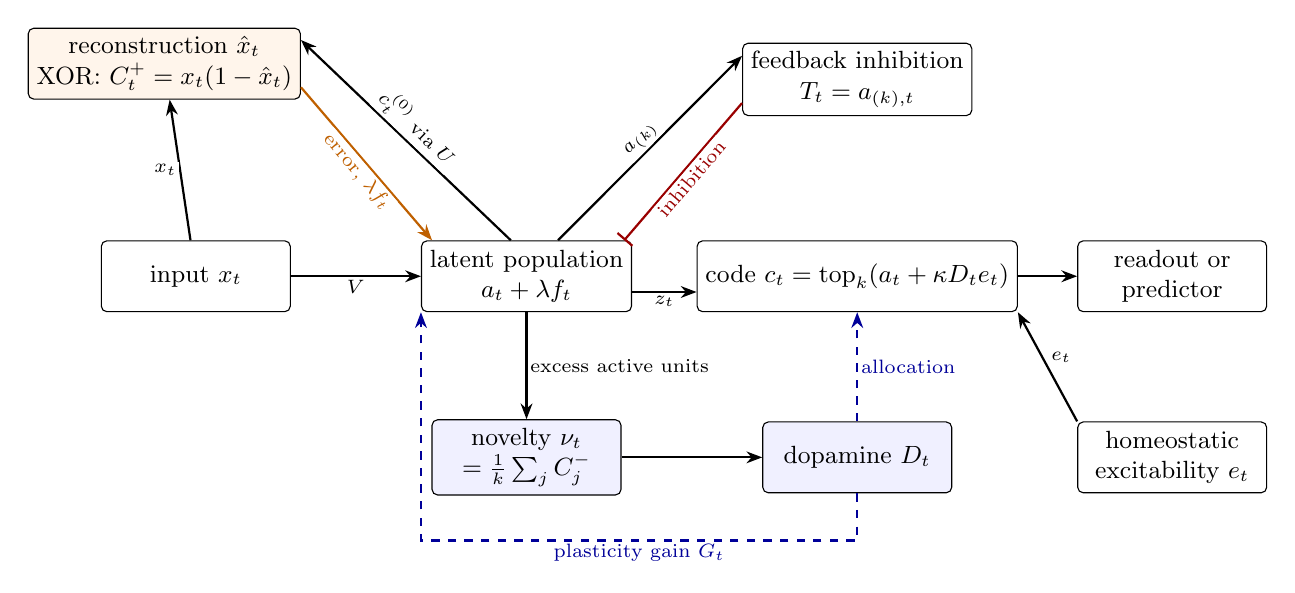
\begin{tikzpicture}[
  box/.style={draw,rounded corners=2pt,align=center,font=\small,minimum height=9mm,minimum width=24mm,inner sep=3pt,fill=white},
  mod/.style={box,fill=blue!6},
  err/.style={box,fill=orange!8},
  lab/.style={font=\scriptsize,fill=white,inner sep=1pt},
  ar/.style={-{Stealth[length=2mm]},thick},
  fb/.style={-{Stealth[length=2mm]},thick,orange!75!black},
  da/.style={-{Stealth[length=2mm]},thick,dashed,blue!60!black}]
\node[box] (in)   at (0,0)     {input $x_t$};
\node[box] (lat)  at (4.2,0)   {latent population\\$a_t+\lambda f_t$};
\node[err] (rec)  at (-0.4,2.7)   {reconstruction $\hat x_t$\\XOR: $C^+_t=x_t(1-\hat x_t)$};
\node[box] (inh)  at (8.4,2.5) {feedback inhibition\\$T_t=a_{(k),t}$};
\node[box] (code) at (8.4,0)   {code $c_t=\topk(a_t+\kappa D_te_t)$};
\node[box] (out)  at (12.4,0)  {readout or\\predictor};
\node[mod] (nov)  at (4.2,-2.3)  {novelty $\nu_t$\\$=\tfrac1k\sum_jC^-_j$};
\node[mod] (da)   at (8.4,-2.3){dopamine $D_t$};
\node[box] (hom)  at (12.4,-2.3){homeostatic\\excitability $e_t$};
\draw[ar] (in)--node[lab,below]{$V$}(lat);
\draw[ar] (in)--node[lab,left]{$x_t$}(rec);
\draw[ar] ([xshift=-2mm]lat.north)--node[lab,above,sloped]{$c^{(0)}_t$ via $U$}([yshift=3mm]rec.east);
\draw[fb] ([yshift=-3mm]rec.east)--node[lab,below,sloped]{error, $\lambda f_t$}([xshift=-12mm]lat.north);
\draw[ar] ([xshift=4mm]lat.north)--node[lab,above,sloped]{$a_{(k)}$}([yshift=3mm]inh.west);
\draw[-{Bar[width=2.5mm]},thick,red!60!black] ([yshift=-3mm]inh.west)--node[lab,below,sloped]{inhibition}([xshift=-1mm]lat.north east);
\draw[ar] ([yshift=-2mm]lat.east)--node[lab,below]{$z_t$}([yshift=-2mm]code.west);
\draw[ar] (code)--(out);
\draw[ar] (lat)--node[lab,right]{excess active units}(nov);
\draw[ar] (nov)--(da);
\draw[da] (da)--node[lab,right]{allocation}(code);
\draw[ar] (hom.north west)--node[lab,above right]{$e_t$}(code.south east);
\draw[da] (da.south) -- ++(0,-0.6) -| node[lab,pos=0.25,below]{plasticity gain $G_t$} (lat.south west);
\end{tikzpicture}
\caption{ENGRAMMER-DOPA. The feedforward drive forms a provisional sparse code, and the inhibition it recruits is set at the level of its $k$-th unit. The code reconstructs the input; a signed-XOR comparison marks the input bits left unexplained ($C^+$). This XOR output reaches the latent layer, where it instructs plasticity and, in the model, also drives activity through the same afferent weights. A learned input is reconstructed and only the $k$ code units are active. A new input leaves error, which excites further units above the inhibition. Their number, the summed depression channel of a signed-XOR comparison between response and provisional code, is the novelty signal. Novelty-evoked dopamine amplifies homeostatic intrinsic excitability, so that rarely used units win the code (allocation), and may increase plasticity. All weights learn by signed-XOR.}\label{fig:concept}
\end{figure}

%======================================================================
\section{A synthetic world: distinguishing novelty from surprise}\label{sec:toy}

\subsection{Experimental design}
\paragraph{Why this experiment is useful.}
In a natural sequence, an event may be unfamiliar because its \emph{identity} is new, or unexpected because its \emph{position in the sequence} is new. We construct a small world in which these cases can be controlled independently. This lets us compare the proposed novelty signal with transition surprise and then ask whether the timing of the modulatory pulse helps protect existing representations.

\paragraph{World and network.}
Each item is a binary pattern with 20 active bits among $D=200$. Initially the world has 30 familiar items connected by a transition graph. Of those items, 70\% have one fixed successor; the other 30\% branch randomly among three successors. There is also a probability of 0.05 per step of jumping to a random item. Input presentations are noisy: an active bit is preserved with probability 0.8, while lost bits are replaced by randomly chosen active bits. Thus familiar inputs will not always be reconstructed without error.

The network has a tied autoencoder with $N=400$ latent units and $k=5$ coding units. Inhibition is fixed at the drive of the $k$-th initial winner. The parameters are $\lambda=0.2$, $\eta=0.02$, $c^-=0$, $\eta_W=0.2$, $\vartheta=0.5$, and $\beta=8$. We first train the world for 6{,}000 steps without modulation. We then compare the different modulatory conditions over the \emph{same} 9{,}000-step test stream, starting from the same trained network for every condition of a seed.

During testing, 15 genuinely new items are inserted into deterministic chains, one every 500 steps. Each shares 40\% of its active bits with an existing familiar item (the \emph{parent}), making interference likely. We also rewire six existing transitions between familiar items. Finally, one-off random inputs that will never recur are shown with probability 0.005 per step. Allocation has $\kappa=0.5$ and $n_0=20$; the optional plasticity gain has $\beta_G=3$.

\paragraph{Choosing a novelty threshold without using performance.}
Because presentation noise creates some reconstruction error even for known inputs, a pulse should not fire on every small excess. Before comparing memory outcomes, we selected the smallest threshold among $\nu_{\rm th}\in\{2,4,8\}$ exceeded by no more than 3\% of familiar presentations. The observed false-alarm rates were 16\%, 7.4\%, and 2.6\%, respectively. The selected value, $\nu_{\rm th}=8$, means that a pulse requires more than 40 additional active neurons beyond the five-neuron code.

\paragraph{Outcomes and controls.}
Every 250 steps, we evaluate the network using noise-free inputs. A \emph{collision} occurs if, at the end of the test, a new item's five-neuron code overlaps its parent's code in at least three neurons. \emph{Stability} is the overlap between a familiar item's current and pre-test codes, averaged across evaluations. \emph{Prediction error} is the Hamming distance between the predicted and actual next codes, divided by $2k$; we report it for transitions involving new items and for unchanged familiar transitions.

The full allocation-plus-gain action is applied (i) when novelty exceeds threshold, (ii) at the same number of times shuffled randomly, (iii) at the same number of highest-surprise times in the unmodulated run, (iv) when the count of unexplained input bits exceeds 8, (v) on the true first presentation of each new or one-off input (an oracle), or (vi) at every step. We also test allocation alone and gain alone. In addition, a causal surprise threshold and fixed-time single-action ablations are reported below. All results use 20 matched random seeds. Differences between conditions are paired, with 95\% bootstrap intervals.

\subsection{Result 1: novelty follows unfamiliar inputs, not unexpected transitions}
When a new item first appears, an average of 116 \emph{additional} latent neurons respond; a one-off random input recruits 140. On later presentations, the excess for new items falls to 8.9, close to the 7.1 extra neurons recruited by noisy presentations of familiar items (Figure~\ref{fig:toy}a). After a single exposure, the response to a newly introduced item therefore returns close to the familiar level. Noise produces some excess on 69\% of familiar presentations, but only 2.6\% cross the selected dopamine threshold.

Crucially, changing the order of familiar items does not have the same effect. Stochastic branches, random jumps and rewired transitions give mean excess counts of 4.4, 5.0, and 4.8. Random jumps and stochastic branches, however, \emph{are} surprising to the transition predictor (rewired transitions are not: 17.5 nats, against 20.0 for familiar presentations). Surprise is 51.2 nats after a random jump between familiar items, almost identical to 50.6 nats on the first appearance of a new item, and 38.9 after a stochastic branch (Figure~\ref{fig:toy}b). Against familiar presentations, the novelty measure detects first presentations with AUC 0.999 $[0.998,0.999]$, compared with 0.886 $[0.872,0.899]$ for transition surprise.

\paragraph{How similar can an unfamiliar input be to a known one?}
For probes that share at most 30\% of their active bits with a familiar item, the median number of active neurons is 119--134 and none is identified as familiar (Figure~\ref{fig:toy}c). At 40\% overlap the median is 95. At 50\% it is 43, with 5\% identified; at 60\% it is 11, with 24\% identified. At 70--80\% overlap the median is 5--6, with 42--56\% identified. Identification therefore changes sharply as a probe becomes similar enough to a stored item. At $\lambda=0.2$, the criterion is deliberately strict.

\begin{figure}[t]\centering
\maybeincludegraphics[width=\textwidth]{fig_v081_toy.pdf}
\caption{Synthetic world, full loop (20 seeds; means $\pm$ s.e.m.). (a) Latent units active beyond the code and (b) transition surprise, for each kind of event during the test. (c) Active units for probes sharing a given fraction of active bits with a familiar item (median and interquartile range). (d--f) The same dopaminergic actions applied at different times, for new items sharing 40\% of their input with a familiar parent: (d) fraction of new items whose code collides with the parent's; (e) stability of the parent's code; (f) prediction error on transitions into and out of new items. Error count: actions applied when more than 8 input bits are unexplained.}\label{fig:toy}
\end{figure}

\subsection{Result 2: acting at the right time separates similar memories}
\paragraph{Comparison with no modulation.}
The difficulty in this world is that a new item resembles an already stored parent. Without modulation, 30\% of new items end with a code colliding with that parent's code (Table~\ref{tab:toy}; Figure~\ref{fig:toy}d). When novelty triggers \emph{both} the allocation bias and the plasticity gain, the actions occur on only 141 of the 9{,}000 test steps, and collisions fall to 2\%. The paired difference is $-0.28$ $[-0.33,-0.23]$. Prediction error falls on transitions involving new items ($-0.033$ $[-0.043,-0.024]$) and on familiar transitions ($-0.025$ $[-0.044,-0.006]$). There is a cost: the familiar parent's code becomes somewhat less stable, 0.76 instead of 0.81 (difference $-0.057$ $[-0.074,-0.041]$).

\paragraph{Why allocation and gain must be combined in this setting.}
When triggered separately by novelty, gain alone leaves 19\% collisions, and allocation alone leaves 9\%. However, these runs generate different subsequent novelty signals and therefore different numbers of triggers. At \emph{exactly the same trigger times} as the combined condition, either action alone leaves 24\% collisions, compared with 2\% for the combination. The paired differences are $-0.22$ $[-0.29,-0.16]$ against allocation alone and $-0.22$ $[-0.26,-0.18]$ against gain alone. The interpretation is specific to the low base learning rate: allocating unused neurons briefly is not enough unless they learn the new input rapidly, while increasing plasticity without reallocating neurons often reinforces the parent's existing code.

\paragraph{Why the timing matters.}
Shuffling the same 141 pulses leaves 20\% collisions and familiar stability of 0.68. Novelty timing is better by $-0.18$ $[-0.23,-0.14]$ for collisions, $+0.075$ $[+0.049,+0.100]$ for parent stability, and $-0.088$ $[-0.102,-0.075]$ for prediction error. Triggering at the 141 highest-surprise times also fails to target learning correctly: collisions remain at 18\%, familiar stability falls to 0.64, and prediction is worse ($+0.066$). This rate-matched surprise condition identifies the most surprising steps \emph{retrospectively} in the unmodulated run. A separate \emph{causal} trigger---surprise more than two running standard deviations above its running mean---fires on 474 steps, leaves 23\% collisions, and reduces parent stability to 0.58. The problem is that surprise repeatedly responds to transitions among known items. Applying both actions at every step prevents most collisions (5\%) but reduces familiar stability to 0.42.

\paragraph{What happens if we trigger directly on reconstruction error?}
The number of missed input bits is a strong detector of first presentations: AUC 0.990 $[0.989,0.990]$, versus 0.999 for latent excess in an unmodulated test with the same seeds. But as a \emph{trigger} in this noisy world, a threshold of more than 8 missed bits fires 1{,}648 times, chiefly during noisy familiar presentations. It reduces collisions to 7\% while lowering parent stability to 0.39 (difference $-0.37$ $[-0.41,-0.33]$ relative to novelty timing); prediction error involving new items rises to 0.56. At thresholds of 4 or 2 missed bits, actions occur on 73--95\% of steps, resembling allocation at every step.

The source of the false alarms is visible in the input comparison. A noisy presentation of a familiar item leaves on average 7.3 of its 20 active bits unexplained; 27\% of these presentations leave more than 8 and 9\% leave more than 12. The first presentation of a new item, by comparison, leaves a median of 20 unexplained bits (minimum 11). A higher raw-error threshold might reduce false alarms, but was not tested as an allocation trigger and was not shown to reach the 2.6\% false-alarm rate of latent excess. One possible explanation is that random noisy bits are dispersed across latent neurons, whereas the missed bits of a new item jointly excite a larger, coherent population. This remains an interpretation, not a separately tested mechanism.

\paragraph{Perfect detection is not necessarily perfect allocation.}
An oracle that pulses on the exact first appearances of new items and one-off inputs leaves 9\% collisions and preserves familiar stability at 0.81. The real novelty signal produces still fewer collisions ($-0.067$ $[-0.100,-0.033]$) because it can pulse on subsequent presentations while a new representation is still being learned. That benefit comes with some loss of familiar stability relative to the oracle ($-0.053$ $[-0.068,-0.038]$), caused partly by the 2.6\% of familiar presentations that cross threshold. Yet familiar-transition prediction is better than under the oracle ($-0.024$ $[-0.036,-0.011]$): code drift is not necessarily functional forgetting here.

For comparison with version 0.7.2, we also reran its feedforward novelty rule using the present code: $\lambda=0$, $T_t=\gamma\max a$ with $\gamma=0.85$, $c^-=0.5$, and $\nu_{\rm th}=1$. That older rule detects first presentations with AUC 0.986 and leaves 5\% collisions after novelty-triggered intervention. Because several components differ, this is a version-level comparison, not an isolated test of feedback.

\begin{table}[t]\small\centering
\caption{Synthetic world, full loop, new items sharing 40\% of their input with a familiar parent: means over 20 seeds. Triggers: number of steps on which the actions were applied (of 9{,}000). Collisions: fraction of new items whose code shares $\ge3$ of 5 units with the parent's. Stability: parent code overlap with its pre-test code. Prediction: error on transitions into and out of new items, and on familiar transitions.}\label{tab:toy}
\begin{tabular}{@{}lccccc@{}}
\toprule
Condition & triggers & collisions & stability & \multicolumn{2}{c}{prediction error} \\
\cmidrule(l){5-6}
 & & & & new & familiar \\
\midrule
no modulation & 0 & 0.30 & 0.81 & 0.30 & 0.20 \\
plasticity gain only (novelty) & 218 & 0.19 & 0.80 & 0.31 & 0.21 \\
allocation only (novelty) & 419 & 0.09 & 0.80 & 0.35 & 0.18 \\
\textbf{allocation + gain, novelty} & 141 & \textbf{0.02} & 0.76 & \textbf{0.27} & \textbf{0.17} \\
allocation + gain, shuffled times & 141 & 0.20 & 0.68 & 0.36 & 0.23 \\
allocation + gain, surprise times & 141 & 0.18 & 0.64 & 0.34 & 0.22 \\
allocation + gain, error count $>8$ & 1648 & 0.07 & 0.39 & 0.56 & 0.57 \\
allocation + gain, oracle times & 60 & 0.09 & 0.81 & 0.27 & 0.20 \\
allocation + gain, every step & 9000 & 0.05 & 0.42 & 0.61 & 0.63 \\
\bottomrule
\end{tabular}
\end{table}

%======================================================================
\section{Class-incremental learning of handwritten digits}\label{sec:mnist}

\subsection{Experimental design}
MNIST adds a complication absent from the synthetic world: two images of the \emph{same class} can differ substantially. Consequently, novelty may mark a new exemplar rather than a new class. The question is whether novelty-controlled allocation helps continual learning under this more realistic form of variability.

Images are binarised at 0.5 and max-pooled to $14\times14$, giving 196 input bits, about 39 of them active. We use a tied autoencoder and a signed-XOR class readout (Section~\ref{sec:learning}), with $k=10$, $\lambda=0.2$, $\eta=0.05$, $\eta_y=0.1$, $c^-=0$, and inhibition at the $k$-th winner. The allocation parameters are $\nu_{\rm th}=1$, $\kappa=0.5$, and $n_0=20$. The use count does not decay during a run. We test capacities $N=1000$ and $N=2000$.

Training proceeds through five consecutive blocks, each containing 1{,}000 images and introducing a pair of classes: (0,1), (2,3), (4,5), (6,7), and (8,9). Images are presented once, without explicit task labels or boundary signals. In the \emph{strict} stream, a class disappears from training as soon as its block ends. In the \emph{recurring} stream, half the images in blocks after the first are drawn from older classes. After each block, we test accuracy on 2{,}000 images from all classes seen so far. Forgetting is the mean reduction, over the classes introduced in the first four blocks, between their best earlier and final accuracies.

The main comparison is between no allocation, allocation on novelty, allocation on every image, and allocation at the same novelty-pulse times shuffled within a run. Additional triggers use (i) unexplained input bits above $\epsilon\in\{2,5,10\}$ and (ii) an error made by the class readout. We repeat conditions with and without a reservoir buffer of 500 past images, replaying one stored image and its signed-XOR update per current step without modulation. An unordered image stream provides another reference.

The configuration was chosen on one seed, excluded from the results. The selection compared $c^-\in\{0,0.5\}$, $\lambda\in\{0.05,0.2\}$, and $\nu_{\rm th}\in\{1,2,4\}$, maximising the mean final accuracy of novelty allocation across four streams. The allocation strength $\kappa$ was not separately optimised for the controls. Results below are for ten additional seeds.

\subsection{Results: allocation helps, but novelty timing depends on recurrence}
\paragraph{Without allocation.}
In a strict sequence of class pairs, the unmodulated network ends at 0.19 accuracy across all ten digits: it mostly remembers the final two classes (Table~\ref{tab:mnist}; Figure~\ref{fig:mnist}a). Mean forgetting reaches 0.95. With $N=2000$, only about 64 neurons are ever recruited into a code. Previously tuned neurons keep beating unused neurons when new classes arrive, so earlier representations are overwritten. Triggering allocation only after a classification error partly mitigates the problem (accuracy 0.49), but this trigger occurs on just 9\% of images, after competition has already selected the representation.

\paragraph{Allocation changes the competitive dynamics.}
In the strict stream, allocating neurons---on novelty, at shuffled times or on every image---improves final accuracy from 0.19 to 0.74--0.89 and reduces forgetting from 0.95 to 0.05--0.25. With novelty triggering, a pulse occurs on 56--67\% of images. At $N=2000$, every unit is eventually used. Thus allocating underused neurons is valuable even in conditions where novelty is \emph{not} the best trigger.

\paragraph{When older classes recur, novelty timing is best.}
For $N=1000$, novelty-controlled allocation reaches accuracy 0.85. This exceeds allocation on every image (0.80; paired difference $+0.049$ $[+0.045,+0.053]$) and at shuffled times (0.81; $+0.041$ $[+0.034,+0.048]$; Figure~\ref{fig:mnist}b). At $N=2000$, novelty reaches 0.88, versus 0.84 for every image ($+0.038$ $[+0.030,+0.046]$) and 0.86 at shuffled times ($+0.013$ $[+0.007,+0.018]$). Allocation on a returning old image may waste neurons by storing another code for something already learned; detecting familiarity avoids some of this duplication.

\paragraph{Replay gives a similar advantage.}
With a buffer of 500 images in the strict stream at $N=2000$, novelty allocation reaches 0.90. This exceeds allocation on every image (0.85; $+0.050$ $[+0.046,+0.054]$), shuffled allocation (0.89; $+0.009$ $[+0.006,+0.013]$), and replay alone (0.65; Figure~\ref{fig:mnist}c). It matches novelty allocation on an unordered stream (0.90), while the unordered stream without allocation reaches 0.68. Replay makes older material recur, so the advantage of avoiding needless new codes is relevant again.

\paragraph{If an old class never returns, novelty is not the best timing rule.}
In the strict stream, novelty allocation performs worse than shuffled allocation: by $-0.019$ $[-0.032,-0.004]$ with $N=1000$ and $-0.051$ $[-0.067,-0.034]$ with $N=2000$. It is also worse than allocation on every image: $-0.032$ $[-0.042,-0.019]$ and $-0.021$ $[-0.041,0.000]$, respectively. Here each new MNIST exemplar can contribute useful variation to a class representation. Spending additional neurons on exemplars may improve classification, even if they are individually similar to previously seen images. This is a boundary of H2, not an effect we exclude from the results.

\paragraph{Is the latent signal more useful than counting error bits?}
At an error-count threshold $\epsilon=5$ the pulse rate is similar to novelty, 57--68\% of images. The resulting accuracies are 0.73 and 0.89 in the strict stream ($N=1000,2000$), and 0.84 and 0.87 in the recurring stream, compared with 0.74, 0.84, 0.85, and 0.88 for novelty. The two triggers are broadly comparable, except that the raw count is better in the strict $N=2000$ case, where it behaves similarly to shuffled allocation.

The signal is a detector of individual inputs, not an oracle for class labels. In the recurring stream with $N=1000$, new-class images exceed the novelty threshold on 87\%, 73\%, 60\%, and 69\% of their presentations in blocks 2--5. Recurring old-class images cross it on 40\%, 58\%, 60\%, and 53\%. Class separation is clear in blocks 2 and 3 but largely disappears by blocks 4 and 5. Literally replayed images, however, cross the threshold on only 18\% of presentations, versus 57--87\% for the new-class images in the corresponding blocks. The difference helps explain why novelty timing works well with exact replay.

\paragraph{Parameter and version controls.}
On the seed used for configuration selection, mean accuracy across the four streams was 0.84 for the selected setting and 0.80 for $\nu_{\rm th}=2$. It was at most 0.39 when $\nu_{\rm th}=4$, $\lambda=0.05$, or $c^-=0.5$, for two different reasons. With $\nu_{\rm th}=4$ or $\lambda=0.05$ the pulse almost never fires (on 0.1--0.5\% of images in the evaluation seeds), and accuracy stays close to that without modulation (0.19--0.63). With $c^-=0.5$ the pulse fires on 18--31\% of images and every unit is eventually used, yet accuracy collapses: the depression of excess units, not a lack of allocation, is the cause. The useful range of the threshold in MNIST is therefore narrow, and the weak feedback gain that works for melodies ($\lambda=0.05$, Section~\ref{sec:songs}) leaves the detector almost silent here. Adding plasticity gain $\beta_G=3$ reduced accuracy in every stream by 0.02--0.05; the base learning rate of 0.05 was already high enough for strong single-presentation updates. The earlier feedforward version 0.7.2 reached 0.50 in the strict $N=2000$ case, 0.80 in recurring $N=1000$, and 0.84 with replay, compared with 0.84, 0.85, and 0.90 in the present full-loop configurations. Since the newer version also disables excess-unit depression ($c^-=0$), this improvement must not be ascribed to feedback in isolation.

\begin{table}[t]\small\centering
\caption{Class-incremental MNIST, signed-XOR learning only, full loop: final accuracy over the ten classes, means over ten seeds (95\% bootstrap intervals in the text). Strict: classes never return. Recurring: half of each later block from earlier classes. Unordered streams ($N=2000$): 0.68 without allocation, 0.90 with novelty allocation.}\label{tab:mnist}
\begin{tabular}{@{}lcccc@{}}
\toprule
& \multicolumn{2}{c}{strict} & \multicolumn{2}{c}{recurring} \\
\cmidrule(lr){2-3}\cmidrule(lr){4-5}
Allocation trigger & $N=1000$ & $N=2000$ & $N=1000$ & $N=2000$ \\
\midrule
none & 0.19 & 0.19 & 0.59 & 0.62 \\
classification error & --- & 0.49 & --- & --- \\
every image & \textbf{0.77} & 0.86 & 0.80 & 0.84 \\
shuffled novelty times & 0.76 & \textbf{0.89} & 0.81 & 0.86 \\
error count ($\sum C^+>5$) & 0.73 & \textbf{0.89} & 0.84 & 0.87 \\
novelty & 0.74 & 0.84 & \textbf{0.85} & \textbf{0.88} \\
\midrule
replay only & & 0.65 & & \\
every image + replay & & 0.85 & & \\
shuffled + replay & & 0.89 & & \\
novelty + replay & & \textbf{0.90} & & \\
\bottomrule
\end{tabular}
\end{table}

\begin{figure}[t]\centering
\maybeincludegraphics[width=\textwidth]{fig_v081_mnist.pdf}
\caption{Class-incremental MNIST with signed-XOR learning only, full loop (ten seeds; means $\pm$ s.e.m.). (a,b) Accuracy on the classes seen so far after each block: (a) strict stream, $N=2000$; (b) recurring stream, $N=1000$. (c) Final accuracy with a 500-image replay buffer; dash-dotted lines, the unordered stream without (grey) and with (blue) novelty allocation.}\label{fig:mnist}
\end{figure}

%======================================================================
\section{Sequential learning of melodies}\label{sec:songs}

\subsection{Experimental design}
This experiment asks two complementary questions. First, can reconstruction feedback make a \emph{frozen random} representation reveal which inputs have been learned, even though the encoder itself never adapts? Second, if the encoder is allowed to learn, can novelty-controlled allocation stop new melodies from reusing the neurons that already encode older melodies? We also ask whether counting unexplained input bits would work equally well.

\paragraph{Data and task.}
We use the sequence-memory corpus of \citet{pena2026songs}: 50 monophonic children's melodies in 4/4 time and 12 held-out melodies. Each beat contains a 12-way one-hot pitch and a two-way onset/sustain value. The network receives three bars (12 beats) as context and predicts the next bar. The main input contains pitch alone: 144 binary lines, 12 active. We also replicate the experiment using pitch and onset together: 168 lines, 24 active. The target bar has 56 binary outputs (pitch and onset at four beats). The training corpus contains 293 contexts; the held-out set has 72. Held-out contexts are distinct from training contexts but can be similar: their median overlap with the most similar training context is 62\% of active bits.

Training is \emph{sequential}: the model learns all contexts of one melody, then moves to the next and never explicitly revisits the previous melody. Each melody is presented in random context order for either 10 passes or 2 passes. The latent layer has $N=4096$ neurons and a code of $k=8$, with inhibition at the $k$-th initial winner unless we state a different control. The next-bar readout learns with $\eta_y=0.1$ from the final code.

\paragraph{Two encoder architectures.}
The \emph{frozen encoder} has random weights drawn uniformly from $[0,1]$. Its separate decoder $U$ learns context reconstruction at $\eta=0.2$; the random feedforward weights do not change. This resembles the random-expansion substrate of \citet{pena2026songs}, but with a simpler output readout. The \emph{plastic autoencoder} ties encoder and decoder weights, initially uniform in $[0,0.3]$, and updates them through signed-XOR with $\eta=0.1$ and $c^-=0$.

\paragraph{How we measure memory.}
\emph{Acquisition} measures teacher-forced next-bar pitch accuracy immediately after each melody is learned. \emph{Retention} measures teacher-forced accuracy across all 50 training melodies at the \emph{end} of the complete sequence, using the correct context. \emph{Free recall} begins with the first three true bars and then generates the remaining bars using its own previous output; the metric is pitch accuracy over generated beats. All final evaluations use the unmodulated code $\topk(a)$. None of these three metrics measures generalisation to genuinely new melodies.

\paragraph{Allocation conditions and statistics.}
The primary dopamine-like pulse fires whenever at least one extra latent neuron is active, $\nu_t>0$. We set $\kappa=0.5$ and $n_0=20$, without use-count decay, and use no plasticity gain except in its explicit ablation. Controls include no allocation, novelty pulses shuffled in time while preserving their exact number, allocation at every step, and allocation triggered by any missed input bit ($\sum_i C^+_{i,t}>0$), along with a shuffled control for those error-count pulses. The comparisons use 30 seeds; differences are paired with 95\% bootstrap intervals, and mean results are accompanied by standard errors where plotted.

\subsection{Result 1: feedback reveals novelty even in a random latent layer}
\paragraph{What happens without feedback?}
With frozen random weights, the feedforward-only rule based on inhibition $T=\gamma\max a$ at $\gamma=0.85$ activates a median of 93 neurons for learned contexts and 95 for held-out contexts. Their activity densities are therefore almost indistinguishable: AUC 0.505 (Table~\ref{tab:songs_det}). Replacing this inhibition with $T=a_{(k)}$ gives exactly eight active neurons for \emph{every} input when feedback is off. That restores sparsity, but the excess-activity signal is then always zero (AUC 0.500). Neither feedforward arrangement detects novelty in the random encoder.

\paragraph{What changes when error returns?}
With inhibition held at the $k$-th feedforward winner, increasing $\lambda$ makes held-out contexts recruit more neurons, while learned contexts remain sparse. The median number of active neurons for held-out contexts is 13 at $\lambda=0.02$, 27 at 0.05, 78 at 0.1, and 336 at 0.2 (Figure~\ref{fig:songs}a). In each case 98--99\% of learned contexts still activate exactly eight neurons. Detection AUC is 0.980 at $\lambda=0.02$, rising through 0.996 and 0.999 to 1.000 at the larger gains. In particular, with $\lambda=0.05$ the familiar response is eight neurons and the novel response has median 27, giving AUC 0.996.

The effect is not confined to eight-neuron codes. At $\lambda=0.05$, using $k=4$, 16, or 32 leaves 97--99\% of learned contexts exactly sparse, with AUC between 0.98 and 0.99. Under $T=\gamma\max a$, sufficiently strong feedback can also separate new contexts (AUC 0.95--0.98 for $\lambda\ge0.1$), but only on top of an already dense baseline of 93 active neurons. As a control, we let $C^-$ excite the latent units as well ($\lambda=0.2$). This is non-physiological if, as in the signed-XOR motif, $C^-$ is carried by inhibitory neurons (Section~\ref{sec:model}). It yields AUC 0.998 but reduces exactly sparse learned contexts to 80\%; false reconstructed bits now also excite the population.

Although the encoder is frozen, its learned output readout retains 0.86 teacher-forced pitch accuracy across the melodies and reaches 0.61 in free recall. The novelty detector therefore does not require encoder plasticity, and the frozen representation is also a meaningful memory baseline.

\begin{table}[t]\small\centering
\caption{Melodies, frozen random latent layer ($N=4096$, $k=8$, pitch-only context): median number of active units for learned (training) and new (held-out) contexts after sequential training, fraction of learned contexts with exactly $k$ active units, and area under the ROC curve of $\nu$ for new against learned contexts. Means over 30 seeds of the per-seed values.}\label{tab:songs_det}
\begin{tabular}{@{}llcccc@{}}
\toprule
Inhibition & feedback gain $\lambda$ & learned & new & exactly $k$ & AUC \\
\midrule
$\gamma\max a$ & 0 (feedforward) & 93 & 95 & 0.00 & 0.505 \\
 & 0.05 & 93 & 207 & 0.00 & 0.853 \\
 & 0.2 & 93 & 974 & 0.00 & 0.983 \\
\midrule
$a_{(k)}$ & 0 (feedforward) & 8 & 8 & 1.00 & 0.500 \\
 & 0.02 & 8 & 13 & 0.99 & 0.980 \\
 & 0.05 & 8 & 27 & 0.98 & 0.996 \\
 & 0.1 & 8 & 78 & 0.98 & 0.999 \\
 & 0.2 & 8 & 336 & 0.98 & 1.000 \\
 & 0.2, $C^-$ also fed back & 8 & 344 & 0.80 & 0.998 \\
\bottomrule
\end{tabular}
\end{table}

\subsection{Result 2: novelty-controlled allocation prevents assimilation of old melodies}
\paragraph{Why plasticity alone fails.}
A plastic encoder could, in principle, learn more efficient representations than a frozen random encoder. In practice, when melodies are learned one after another without allocation, the early winning neurons keep winning. Only 107 of the 4{,}096 neurons are ever used; just 35\% of learned contexts finish with exactly eight active units. Importantly, the individual melodies \emph{are} acquired when presented (acquisition 0.99), but are later overwritten: final teacher-forced retention is 0.36 and free recall is 0.27 (Table~\ref{tab:songs_alloc}; Figure~\ref{fig:songs}b). This is sequential interference, not a failure to fit the current melody.

\paragraph{What novelty-timed allocation changes.}
With feedback gain $\lambda=0.2$, novelty triggers a pulse on 24\% of training steps. These pulses bring 1{,}808 neurons into use; 97\% of learned contexts end with exactly eight active neurons. Retention rises to 0.92 and free recall to 0.87. The \emph{same number} of pulses shuffled in time recruits fewer neurons (1{,}325) and reaches only 0.64 retention and 0.49 free recall. The paired differences are $+0.280$ $[+0.272,+0.288]$ and $+0.379$ $[+0.369,+0.391]$, respectively. Thus both the allocation action and its timing matter in this setting.

Compared with the frozen representation, novelty allocation in the plastic encoder improves retention by $+0.067$ $[+0.061,+0.072]$ and free recall by $+0.262$ $[+0.248,+0.275]$. With weaker feedback, $\lambda=0.05$, novelty fires on 16\% of steps and reaches 0.85 retention, against 0.61 for the same pulses shuffled (difference $+0.233$ $[+0.225,+0.241]$). Allocation at \emph{every} step reaches 0.95 retention, slightly above novelty's 0.92 (difference for novelty $-0.024$ $[-0.030,-0.020]$), but requires about four times as many pulses. Adding plasticity gain $\beta_G=3$ to novelty allocation \emph{reduces} retention to 0.87 (difference $-0.050$ $[-0.056,-0.044]$). As in MNIST, accelerating an already effective learning update can increase interference.

\paragraph{The two-pass limit.}
The preceding benefit depends on presenting each melody enough times for its plastic code to settle. With only two passes per melody, novelty is detected on 88\% of steps; all allocation strategies reach only 0.64--0.67 retention. The frozen layer retains 0.86, outperforming novelty-allocated plastic learning by 0.189 (difference reported for novelty $-0.189$ $[-0.196,-0.181]$). Allocation still helps relative to no modulation (0.37), but it cannot substitute for sufficient learning of each code. The correct inference is conditional: plasticity plus appropriate allocation can outperform a frozen random encoder \emph{if the new representations are adequately trained}.

\begin{table}[t]\small\centering
\caption{Melodies, tied plastic autoencoder ($\lambda=0.2$, $k=8$, pitch-only context): teacher-forced retention and free recall over the 50 melodies after sequential training, fraction of steps with a dopamine pulse, number of units ever used in the code, and fraction of learned contexts with exactly $k$ active units. 30 seeds; the frozen random layer is shown for reference. Shuffled controls use exactly the pulses of the corresponding trigger, permuted in time.}\label{tab:songs_alloc}
\begin{tabular}{@{}lccccccc@{}}
\toprule
& \multicolumn{5}{c}{10 passes per melody} & \multicolumn{2}{c}{2 passes} \\
\cmidrule(lr){2-6}\cmidrule(l){7-8}
Dopamine pulses & retention & free & pulses & units & exactly $k$ & retention & pulses \\
\midrule
none & 0.36 & 0.27 & 0 & 107 & 0.35 & 0.37 & 0 \\
novelty, shuffled & 0.64 & 0.49 & 0.24 & 1325 & 0.70 & 0.64 & 0.88 \\
\textbf{novelty} ($\nu_t>0$) & \textbf{0.92} & \textbf{0.87} & 0.24 & 1808 & 0.97 & 0.67 & 0.88 \\
error count, shuffled & 0.69 & 0.54 & 0.41 & 1637 & 0.85 & 0.67 & 0.99 \\
error count ($\sum C^+>0$) & 0.97 & 0.94 & 0.41 & 1927 & 0.98 & 0.67 & 0.99 \\
every step & 0.95 & 0.90 & 1 & 2185 & 0.99 & 0.67 & 1 \\
novelty, with plasticity gain & 0.87 & 0.78 & 0.12 & 1521 & 0.94 & 0.62 & 0.46 \\
\midrule
frozen random layer & 0.86 & 0.61 & --- & 1137 & 0.98 & 0.86 & --- \\
\bottomrule
\end{tabular}
\end{table}

\begin{figure}[t]\centering
\maybeincludegraphics[width=\textwidth]{fig_v081_songs.pdf}
\caption{Sequential learning of 50 children's melodies (30 seeds; pitch-only context). (a) Median number of active latent units for learned (dashed) and new (solid) contexts as a function of the gain $\lambda$ of the returning error, in a frozen random layer, with inhibition set by the strongest unit (grey) or by the $k$-th winner (blue); $k=8$, $N=4096$. (b,c) Teacher-forced retention over the 50 melodies in a tied plastic autoencoder with dopamine pulses at different times, after 10 (b) or 2 (c) passes per melody; the frozen random layer is shown for reference. Random times: the novelty pulses of the same seed, shuffled. Percentages: fraction of steps with a pulse. Means $\pm$ s.e.m.}\label{fig:songs}
\end{figure}

\subsection{Result 3: what does latent excess add to a raw error count?}\label{sec:nu_vs_err}
The proposed signal is produced by the reconstruction error, and a simpler circuit could sum the missed input bits directly: $E_t=\sum_i C^+_{i,t}$. To justify measuring excess \emph{latent} activity, we need to ask whether it provides information or behaviour unavailable from $E_t$. The answer is mixed, and it is important not to conflate the three comparisons below.

\paragraph{Detecting wholly new contexts: no advantage over raw error.}
In the frozen random encoder, the raw missed-bit count separates held-out from learned contexts with AUC 1.000. It is at least as good as the latent signal for this specific detection task. The effect of the error on latent activity does not create previously unavailable information; it makes the information appear as population density in a representation that could influence the selection of coding neurons.

\paragraph{Directing allocation: equivalent at comparable pulse rates.}
At its natural threshold $E_t>0$, raw error pulses on 41\% of steps and gives retention 0.97, versus 0.92 for $\nu_t>0$ with pulses on 24\% of steps (difference for novelty $-0.042$ $[-0.047,-0.037]$). More frequent allocation is itself beneficial, so this is not a fair comparison of timing signals. When thresholds are chosen to give approximately 25\% pulses, both triggers yield 0.92 retention ($\nu>0$ versus $\sum C^+>3$; Figure~\ref{fig:songs_ctrl}a). Near 20\% pulses, novelty retains 0.86 at 18\% of steps, whereas the error count retains 0.81 at 20\%. For either signal, shuffling the pulses reduces retention by approximately 0.28. The central conclusion is \emph{not} that excess activity always outperforms raw error: at matched frequencies, their allocation performance is often the same.

\paragraph{Recognising a noisy version of a learned context: an advantage for latent excess.}
We then modified already learned contexts by deleting, adding, or replacing pitches at one to twelve beats. In the frozen random layer at $\lambda=0.2$, latent excess remains highly sensitive: it flags a one-beat pitch substitution in 99\% of cases. After sequential learning \emph{with novelty allocation}, the two signals behave differently (Figure~\ref{fig:songs_ctrl}b). A single pitch substitution leaves unexplained input bits in every case, yet produces $\nu>0$ in only 9.5\% of cases. Three substitutions are flagged by latent excess in 44\%, and six or more in at least 99.7\%. Similarly, adding one pitch bit is flagged by raw error in every case but by latent excess in only 6\%. The network has acquired tolerance to small changes of known patterns without losing sensitivity to larger changes.

This tolerance does not usually hide truly different held-out contexts. Latent excess flags 100\% of held-out contexts sharing less than 65\% of active bits with the nearest training context and 98\% sharing 65--80\%. Fewer than half of the four held-out contexts above 80\% similarity are flagged. The likely explanation is that learning strengthens the margin between the winning neurons of a familiar code and the neurons below threshold; a few scattered missed bits then fail to recruit new units. This explanation is plausible but not separately established by these experiments.

\paragraph{An important asymmetry: deletion of learned content.}
A missing note is harder to detect, as expected when only $C^+$ recruits units. After learning, deletions are flagged in only 5--25\% of cases by latent excess and 12--28\% by raw error. Letting $C^-$ excite the frozen layer (the non-physiological control) raises detection of a single deletion to 98\% from 85\%, but makes a substantial fraction of learned responses non-sparse (Table~\ref{tab:songs_det}). Thus the present signal is sensitive to \emph{unexplained present bits}, not symmetric mismatch in both directions.

\paragraph{Repeated noisy presentations.}
After ordinary training, we gave each learned context one additional presentation with one pitch substituted, leaving learning and allocation active. Under the raw-error trigger, 99.9\% of these noisy presentations produced pulses and recruited 360 newly used neurons. Under the latent trigger, only 11\% produced pulses, recruiting 131 neurons. Final retention was 0.96 for raw error and 0.93 for latent novelty, with little change because the noisy pass also rehearsed the melodies. Those retention values cannot be interpreted as a clean measure of damage. The synthetic world, where familiar inputs are noisy throughout learning, provides the stronger evidence that excess raw-error triggering can destabilise existing codes.

In summary, the error count is a serious alternative baseline, not a straw man. For clean detection and rate-matched allocation it performs as well as latent excess. The potential additional value of the latent signal is \emph{learned tolerance}: the code can continue to identify slightly altered familiar items without continually reallocating neurons.

\begin{figure}[t]\centering
\maybeincludegraphics[width=\textwidth]{fig_v081_songs_controls.pdf}
\caption{Latent excess against error count (melodies, pitch-only context, 30 seeds). (a) Teacher-forced retention against the fraction of steps with a dopamine pulse, for thresholds on $\nu$ ($0$, $0.5$, $1$, $2$, $4$) and on $\sum C^+$ ($0$, $1$, $2$, $3$, $5$), tied plastic autoencoder; squares, the same pulses shuffled in time; frozen layer and pulses at every step for reference. (b) Fraction of learned contexts flagged as new after substituting the pitch of a given number of beats, in the network trained with novelty allocation (blue, $\nu>0$; orange, $\sum C^+>0$) and in the frozen random layer ($\nu>0$, grey, hidden under the orange line). Means $\pm$ s.e.m.}\label{fig:songs_ctrl}
\end{figure}

\subsection{Replication using pitch and onset}
Including the onset/sustain input bits produces qualitatively similar but less sharply separated responses. In the frozen encoder, AUC for held-out contexts is 0.88--0.95 across $\lambda=0.02$--$0.2$, and only 55--82\% of learned contexts remain exactly sparse. Its retention is 0.70.

For the plastic autoencoder with $\lambda=0.2$, novelty allocation occurs on 34\% of steps and yields 0.87 teacher-forced retention and 0.75 free recall. At exactly the corresponding shuffled times, retention is 0.66 and free recall 0.51; the paired differences are $+0.205$ $[+0.196,+0.213]$ and $+0.239$ $[+0.225,+0.252]$. Without modulation the values are 0.30 and 0.24; with allocation at every step they are 0.88 and 0.78; with the frozen layer they are 0.70 and 0.39. Raw-error triggering achieves 0.90 retention at its natural threshold, with pulses on 49\% of steps. When melodies have only two passes, the frozen layer again wins (0.69 versus 0.58 for novelty allocation). These results repeat the main pattern without implying that pitch-plus-onset inputs behave identically to the simpler pitch-only representation.

\subsection{Interim conclusion across the three experiments}
The evidence supports \emph{allocation} most generally. Without it, a small set of early winning neurons can monopolise new inputs, causing collisions or catastrophic interference despite successful acquisition of individual items. A novelty-triggered allocation pulse alleviates this problem in the synthetic world, MNIST, and melodies, all trained with signed-XOR updates. Once the effect of the XOR output on latent activity is included, learned inputs are sparse and novel ones denser even in an initially random encoder. Importantly, novelty timing outperforms equally frequent shuffled pulses in the synthetic world, the melody experiment, and MNIST when earlier inputs recur or are replayed. It does \emph{not} outperform the controls when earlier MNIST classes disappear permanently. Nor does latent excess universally improve on a raw reconstruction-error count. Its more distinctive advantage is that an adapted encoder tolerates small changes and noise in familiar inputs. Finally, the plasticity gain is helpful only when the baseline update is too weak to establish a new code. All of these qualifications are part of the result.

\section{Predictions for dopamine}\label{sec:predictions}
The simulations do not measure dopamine. They establish that a novelty-sensitive global signal \emph{could} control memory allocation, and propose a specific excitability-based implementation. H3 would require experiments relating dopamine to late population activity, homeostatic excitability, and the overlap of neurons assigned to similar memories. The following predictions distinguish this proposal from accounts based primarily on reward prediction error \citep{schultz1997}, information gain or surprise \citep{beck2026}, or a separate learned familiarity memory \citep{dasgupta2018,kakade2002}. Each prediction includes an observation that would challenge it.

\begin{table}[t]\small\centering
\caption{Predictions and the observations that would refute them.}\label{tab:predictions}
\begin{tabularx}{\textwidth}{@{}P{0.6cm}LL@{}}
\toprule
& Prediction & Refuting observation \\
\midrule
P1 & Novelty-related dopamine scales with the number of active neurons in the upstream sparse population (e.g.\ dentate gyrus, piriform cortex, Kenyon cells) beyond its usual sparseness & novelty responses unrelated to population density at fixed input strength \\
P2 & The novelty response habituates after one or a few exposures, at the rate at which the upstream code becomes sparse & habituation without sparsening, or sparsening without habituation \\
P3 & Unexpected transitions between familiar stimuli do not evoke the novelty response, although they evoke surprise-related signals & a novelty-type response to rearranged familiar stimuli \\
P4 & Novel stimuli increase the number of active neurons in a late component of the response, after the initial feedforward volley; inhibition does not hold the number constant. Familiar stimuli, and partial versions of them, do not & equal numbers of active neurons for novel and familiar stimuli, or an excess already present in the earliest response and unaffected by feedback \\
P5 & Dopamine increases the excitability of rarely used neurons more than that of recently and frequently used ones, in proportion to their homeostatic excitability & a uniform or reversed dopaminergic effect on excitability \\
P6 & Blocking dopamine during the first exposure to a stimulus similar to a familiar one increases the overlap of their engram cells and impairs their discrimination; blocking homeostatic intrinsic plasticity has the same effect & unchanged engram overlap and discrimination \\
P7 & Silencing the projection of the input--reconstruction comparison (the XOR output) to the latent layer abolishes the novelty-related excess and the novelty response of dopamine neurons, but leaves the sparse response to familiar stimuli intact & novelty-related excess or dopamine response unchanged after silencing the feedback \\
\bottomrule
\end{tabularx}
\end{table}

P1 and P2 can be tested by recording the activity of a sparse population together with dopamine during successive exposures to new stimuli. P3 asks whether a surprising \emph{reordering} of familiar stimuli elicits the same putative novelty signal. P4 concerns the time course: a novel stimulus should produce a late increase in population activity following the initial sparse response. In the insect mushroom body, feedback inhibition is provided by an identified interneuron that can be manipulated \citep{lin2014}. P5 and P6 require direct excitability measurements and engram tagging combined with dopaminergic interventions \citep{josselyn2018,yiu2014}. P7 is an especially direct test: interrupting the projection that carries the reconstruction mismatch to the latent layer should abolish the proposed excess response without abolishing the initial sparse response to familiar stimuli.

\section{Discussion}\label{sec:discussion}

\subsection{The main computational result: deciding which neurons will learn}
A local signed-XOR correction can tell a synapse whether to strengthen or weaken. It does not tell the entire population \emph{which neurons should take responsibility} for a new input. Our experiments illustrate why this second decision matters. In a competitive sparse network, an already tuned neuron may win for a new input simply because it has stronger weights than an unused neuron. Its old connections are then rewritten. The model uses a population-level identification signal to decide when to bias the competition in favour of less-used neurons.

This decision does not require storing an additional catalogue of past inputs. Reconstruction error already exists in the autoencoder; its return recruits neurons that were below the inhibition set by the first response. A downstream circuit can count this excess with a simple population-level readout. A scalar modulatory signal can then change the competition across the latent population with a number of operations scaling linearly with its size. This is the proposed benefit of neuromodulation: it decides \emph{where} learning occurs, rather than supplying a better signed-XOR correction at each individual synapse.

The advantage has limits. In all three experiments, allocation itself helps prevent excessive reuse of early winners. Novelty is a particularly useful \emph{timing} rule when genuinely familiar inputs reappear among new ones. It is less useful when a stream continually supplies new exemplars and never returns to old classes, as in the strict MNIST experiment. It also cannot replace sufficient exposures to each new melody. These distinctions make H2 a conditional mechanistic claim, not a universal performance advantage.

\subsection{Why homeostatic excitability is a plausible allocation mechanism}
The model combines two different effects with different time scales. First, repeated use slowly reduces a neuron's intrinsic excitability through homeostatic adaptation \citep{desai1999,turrigiano2008}. Second, a brief dopamine-like signal amplifies the remaining differences in excitability. Under that rule, neurons with little prior use are more likely to win a new representation. Excitability-based allocation agrees qualitatively with experiments showing that relatively excitable neurons are preferentially recruited into engrams \citep{josselyn2018,yiu2014}. The crucial \emph{quantitative} coupling between dopamine and homeostatic excitability, however, remains the hypothesis P5 rather than an established experimental fact.

There is a potentially informative complication. Neurons recruited into a recent memory can remain highly excitable for several hours and be recruited again, thereby linking memories formed close in time \citep{josselyn2018}. A richer model could include a short-lived \emph{increase} in excitability immediately after recruitment, followed by a slower homeostatic \emph{decrease}. Their balance would determine whether successive new experiences share or avoid neurons. The present simulations include only the simpler slow-use mechanism, so they do not model this temporal linking effect.

\subsection{Relation to other models of recognition and memory separation}
The reconstruction-and-comparison stage has a family resemblance to adaptive resonance theory: a top-down template is compared with the input, and insufficient agreement changes how the input is categorised \citep{carpenter1987}. Adaptive resonance commonly resets an insufficiently matching winner and searches for another category. Here the mismatch instead excites \emph{additional} neurons, and the number of these neurons serves as a novelty signal. A modulatory change in competition, rather than a dedicated reset operation, then guides allocation.

An error that projects back to the representation is also the core of predictive coding \citep{rao1999}. The difference is the use made of it. The signed-XOR autoencoder already sends its binary error channels to the latent layer to instruct learning; here the $C^+$ channel is also read through the activity it evokes, which exposes identification failure as population density. It is not used to iteratively refine an estimate of the input. The subsequent allocation produces a form of \emph{pattern separation} \citep{yassa2011}. The hippocampal dentate gyrus is an appealing candidate for testing this idea because its coding is sparse, inhibition is strong, and it interacts with novelty-responsive neuromodulatory systems \citep{lisman2005}. This analogy is suggestive, not evidence that such a projection, or the required inhibition, exists there.

\subsection{The mushroom body as a possible biological test bed}
In the insect mushroom body, Kenyon cells use sparse odour representations constrained by feedback inhibition. Disrupting that inhibition increases population density and makes discrimination of similar odours worse \citep{lin2014}. Novelty-related responses also occur in mushroom-body output neurons and are modified by dopaminergic plasticity at their input synapses \citep{hattori2017}. Those observations show one mechanism for familiarity in the output pathway; they do \emph{not} establish that novel odours recruit more Kenyon cells or that dopamine allocates new Kenyon-cell representations.

Our proposed mechanism makes an additional prediction: a late, reconstruction-dependent component should increase the \emph{number} of active Kenyon cells on novel trials (P1 and P4). A frozen random expansion, as used in the melody experiment, shows that such a population could reveal familiarity \emph{if} the comparison error reaches it. Whether an error projection of this kind exists in the mushroom body is unknown (P7). Likewise, biological inhibition is partly local and input-dependent; if it continually enforces a fixed population size, the mechanism would fail. The signed-XOR motif has been reported as enriched in the \emph{Drosophila} connectome \citep{pena2026motif}, and individual mushroom-body dopaminergic neurons have been identified \citep{aso2016}, providing possible targets for a circuit-level investigation.

\subsection{Relation to earlier signed-XOR melody memory}
The related sequence-memory study \citet{pena2026songs} memorised the same corpus of 50 melodies with a frozen sparse random encoder and a Dale-compliant signed-XOR readout, and found that making its encoder plastic was detrimental. That work could detect novelty from the residual of a teacher-forced \emph{next-bar prediction}. The present work instead compares the \emph{current context} with its reconstruction; it therefore does not require seeing the melody's continuation. These signals address different questions and may coexist.

Our unmodulated plastic-encoder result agrees that sequential encoder learning can be worse than keeping the random encoder fixed. The improvement introduced here arises when novelty helps allocate the new representation to less-used neurons and enough presentations are available to learn it. In that situation, the plastic encoder gives stronger retention and free recall in this experiment. However, the readout used here is substantially simpler than the one in \citet{pena2026songs}; their absolute retention values are \emph{not directly comparable}. Neither the present teacher-forced retention nor free recall metric assesses generalisation to new melodies.

\subsection{What novelty does not say}
Novelty is not the same as utility. A completely unfamiliar but irrelevant, one-off input will also produce a novelty response. In the synthetic world, an oracle pulses on such events as well. In a finite-capacity memory, an allocation to a one-off event must eventually be recovered or pruned. Slow recovery of excitability in inactive neurons provides one possible mechanism; another is requiring re-exposure before an initially tagged trace becomes stable, as in synaptic tagging and capture \citep{frey1997,moncada2007}. The cost is measurable in the synthetic world. One-off random inputs fire a pulse every time: about 45 of the 141 pulses of a test, and 26 of the 101 latent units still unused after familiarisation, against 13 for the new items. The slow decay of the use count is implemented there, but its ability to recover these units was not measured, and re-exposure-dependent consolidation is not implemented. Whether a prior on the structure of the input could keep noise from being allocated is left for future work.

Novelty is also not surprise. Random jumps among familiar items produce strong transition surprise but little identification failure. Earlier experiments on gating signed-XOR consolidation by surprise gave limited benefits (Appendix~\ref{app:surprise}), motivating the present mechanism. But the two signals might still have different useful roles in a richer model. Finally, latent excess is not a guaranteed improvement over raw reconstruction error. Both detect unlearned contexts, and at matched rates both often guide allocation equally well. The observed additional value of excess activity is tolerance to small mismatches \emph{after encoder training}; it remains dependent on the network architecture and its noise regime.

\subsection{Is the modulator necessarily dopamine?}
No. Acetylcholine has been proposed to promote an encoding mode for new hippocampal inputs \citep{hasselmo2006}, and noradrenaline has been linked to unexpected uncertainty \citep{yu2005}. Either could contribute to an identification-dependent change in allocation. We focus on dopamine because of its links to novelty, memory persistence and cellular excitability \citep{duszkiewicz2019,takeuchi2016,durstewitz2008,kutter2026}. The assignment to dopamine is H3 and is \emph{not tested} by any of the simulations. Selective excitability modulation (P5), altered engram overlap when dopamine is blocked (P6), and suppression of the error projection to the latent layer (P7) would be particularly discriminating experiments.

\subsection{Limitations and next steps}
\begin{enumerate}[leftmargin=*]
\item \textbf{Idealised inhibition and timing.} The main result requires an inhibitory level established by the initial $k$ winners and held fixed as error returns. We have not shown that a recurrent excitatory--inhibitory circuit exhibits this behaviour. Replacing Eq.~(\ref{eq:inhib}) with an explicit recurrent circuit is the most important next modelling step. Reconstruction and feedback also introduce delays: the modulatory signal must arrive while the final code is still alterable. Delay tolerance in the present allocation model has not been measured, although earlier consolidation-gating versions examined delay.
\item \textbf{Sensitivity to thresholds and learning rules.} In MNIST, $\lambda=0.2$ and $\nu_{\rm th}\le2$ work, but lower feedback gain, higher threshold or active excess-unit depression can make allocation ineffective. In the synthetic world the novelty threshold must exceed the effects of presentation noise. The experiments use different thresholds---8, 1 and 0---each selected by a stated rule, not a universal setting. The gain $\lambda$, allocation strength $\kappa$, and possible graded dopamine response remain to be studied systematically.
\item \textbf{Limited scale and baselines.} The experiments are small. MNIST uses one architecture, ten evaluation seeds and reduced images; it does not compare against engineered continual-learning systems. The melody task measures memory of the training corpus, not generalisation. More systematic comparisons across capacity, data distributions, stream recurrence and learning rate are needed. A tuned homeostatic utilisation-balancing baseline without novelty is also missing: the tested all-steps allocation control uses the same $\kappa$ as the novelty condition.
\item \textbf{Biological locality.} In the tied autoencoder, the decoder update also changes the feedforward encoder weights. Its decoder form is a signed-XOR correction, but reciprocal encoder synapses would need to share these updates. In addition, the model routes the XOR output to latent activity through the encoder weights, as if the error lines shared the afferent synapses of the input lines. The full model is therefore not yet a strictly local biological circuit. Separate encoder, decoder and feedback pathways with individually local rules should be tested. The frozen encoder with a separate decoder is an initial step in that direction.
\item \textbf{One-sided error detection.} Because only $C^+$ recruits units, the signal often fails to flag a learned input from which part has been deleted. Letting $C^-$ excite as well increases deletion sensitivity, but reduces the fraction of exactly sparse familiar representations, and is non-physiological if $C^-$ is inhibitory. Deletions might instead be read from the inhibitory channel itself, for instance as a deficit of activity in the code; this remains to be designed.
\item \textbf{Allocation and persistence.} Newly assigned neurons are not necessarily consolidated, useful or protected indefinitely. Short-lived novelty, memory importance, re-exposure and available capacity should eventually be modelled as separate variables rather than equated with a single pulse.
\end{enumerate}

%======================================================================
\section{Conclusion}
In this model, an input is novel when its sparse representation fails to explain it. The network does not need to predict the next event to know this. It first reconstructs the current input from a provisional code. The signed-XOR comparison of input and reconstruction projects to the latent population, as it does to instruct learning, and the unexplained input bits also drive latent activity. If the input is already learned, the response remains sparse. If it is not, extra neurons cross the inhibition established by the initial response. Their number is a usable novelty signal, and it can be written as the summed depression channel of a second signed-XOR comparison.

The central learning consequence is a change in \emph{allocation}. A brief dopamine-like pulse biases the final code towards less-used, more excitable neurons, making it harder for a new memory to overwrite a similar old one. This improves separation in a synthetic world and supports sequential memory in MNIST and melodies, with a clear advantage for novelty timing when familiar and novel inputs recur together. The same advantage does not hold when old MNIST classes never reappear. The raw count of unexplained input bits is a strong alternative trigger, and at equal pulse rates can work just as well. Excess latent activity becomes more distinctive after learning, when it tolerates small deviations from familiar inputs. The simulations support H1 and provide conditional evidence for H2. Whether dopamine uses this circuit mechanism---H3---is an experimentally testable hypothesis, not a result of the paper.

\section*{Version note}
Initial versions proposed that the surprise of latent transitions gates the consolidation of signed-XOR corrections; their numerical test was largely negative (Appendix~\ref{app:surprise}). Following versions defined novelty as identification failure, measured on the feedforward response of a trained encoder. Next versions included the effect on latent activity of the XOR output that the signed-XOR autoencoder already projects to its latent layer, which earlier simulations had left out, and set inhibition at the $k$-th winner. Latest versions repeated all experiments with this loop, used 30 seeds for the melodies, and added the comparison with the raw error count, perturbation probes and free recall. 

\section*{Data and code availability}
No new experimental data were generated. The study uses the public MNIST data set and the melody corpus of \citet{pena2026songs}, available at \url{https://github.com/jesusmarcodelucas/musicmem-engrammer}. The simulation code (Python~3, NumPy) that produces all figures and tables in this preprint is deposited in the same public repository, at \url{https://github.com/jesusmarcodelucas/musicmem-engrammer/Dopamine} , together with the configuration-selection scripts. The full set of runs takes about 20 core-hours.

%======================================================================
\appendix
\section{Proofs}\label{app:proofs}
The propositions above concern the response of the \emph{specified} threshold model. They are algebraic properties of the equations, not claims that a biological circuit necessarily implements those equations. Throughout, assume that the feedforward drives are distinct so the ranking of the $k$ strongest units is unambiguous.

\paragraph{Proof of Proposition~\ref{prop:ident}: identification criterion.}
Because $V\ge0$ and $C^+_t\ge0$, the feedback $f_t\ge0$. Hence $a'_{j,t}\ge a_{j,t}$ for all $j$.
\begin{enumerate}[label=(\roman*)]
\item Every member of the provisional code has $a_{j,t}\ge a_{(k),t}=T_t$. It therefore remains active after non-negative feedback. The response consists of these $k$ units plus $k\nu_t$ additional units, giving $|z_t|=k(1+\nu_t)$.
\item For any unit outside that code, $z_{j,t}=1$ exactly when $a_{j,t}+\lambda f_{j,t}\ge a_{(k),t}$, or equivalently when $\lambda f_{j,t}\ge a_{(k),t}-a_{j,t}$.
\item If $C^+_t=0$, then $f_t=0$. With distinct initial drives, no unit outside the provisional code can exceed the $k$-th-winner threshold, so $\nu_t=0$. Conversely, $\nu_t>0$ implies that some unit outside the provisional code satisfies $\lambda f_{j,t}\ge a_{(k),t}-a_{j,t}>0$. Thus $f_{j,t}>0$, which requires $C^+_t\ne0$.
\item Multiplying both $a_t$ and $f_t$ by $s>0$ multiplies each side of every threshold comparison by $s$, without changing the active set. In the special case $\lambda=0$ and $T_t=\gamma a_{(1),t}$, exactly those units outside the top $k$ with $a_{(j),t}\ge\gamma a_{(1),t}$ contribute to the excess.
\end{enumerate}
\hfill$\square$

\paragraph{Proof of Proposition~\ref{prop:sxor}: population signed-XOR identity.}
Let $q_j=c^{(0)}_j$ and $o_j=z_j$ be binary. The expression $(1-q_j)o_j$ is one precisely when $o_j=1$ but $q_j=0$, i.e. when an active unit lies outside the provisional code. Summing these terms gives $k\nu_t$. Similarly, $q_j(1-o_j)$ is one precisely when a provisional code neuron is not active. By Proposition~\ref{prop:ident}(i), this cannot occur when inhibition is set at the $k$-th initial winner. With the alternative $T_t=\gamma\max a$ and $\lambda=0$, if at least $k$ neurons are active, all top-$k$ neurons must be among them; the potentiation channel is then also zero. \hfill$\square$

\paragraph{Proof of Proposition~\ref{prop:equiv}: excitability and use penalty.}
For each neuron let $m_j=\min(u_j/n_0,1)$, so that $e_j=1-m_j$. Then
\[
a_j+\kappa D(1-m_j)=(a_j-\kappa Dm_j)+\kappa D.
\]
The additive term $\kappa D$ is the same for every unit and therefore leaves their rank order unchanged. The $k$-winner code is identical under either scoring rule. \hfill$\square$

\section{Simulation details}\label{app:methods}
The following information specifies the runs reported above. The numerical experiments are those of version 0.8.1.

\subsection{Synthetic world}
\begin{itemize}
\item \textbf{Patterns and transitions.} The initial world contains 30 familiar patterns, each with 20 active bits among 200. Twenty-one items have one successor drawn from the other familiar items; nine items branch uniformly among three fixed options. With probability 0.05 per step, the next item is drawn from all items currently present.
\item \textbf{Changes during testing.} New items indexed $j=0,\dots,14$ are inserted at steps $250+500j$ between a deterministic familiar item and its successor. Six other deterministic items have successors redrawn at steps $500+1300r$. One-off random inputs replace the current item with probability 0.005 per step without advancing the sequence. Each new item shares eight of its 20 active bits with a randomly chosen familiar parent.
\item \textbf{Initialisation and utilisation.} Initial weights are uniform in $[0,0.3]$. The use count decays with time constant $2\times10^4$ steps.
\item \textbf{Control timing.} Shuffled times are a permutation of the novelty triggers of the same seed. The rate-matched surprise condition uses the steps with highest surprise in the unmodulated run, with the same number of pulses as the novelty condition. The oracle pulses on first presentations of new items and all one-off inputs. Raw-error thresholds are more than $\epsilon\in\{2,4,8\}$ missed input bits. For fixed-time action ablations, allocation alone or gain alone occurs at the exact joint-condition novelty times for that seed.
\item \textbf{Parameter selection and seeds.} We use $c^-=0$ and $\lambda=0.2$ from the MNIST selection, while $\nu_{\rm th}\in\{2,4,8\}$ is selected using the familiar-input false-alarm rule in Section~\ref{sec:toy}. Additional runs with $c^-=0.5$ or $\lambda=0.05$ were performed but are not reported as main conditions. Results use seeds 1--20.
\end{itemize}

\subsection{Melody sequences}
\begin{itemize}
\item \textbf{Corpus and inputs.} We use \texttt{songs\_train.json} (50 melodies) and \texttt{songs\_novel.json} (12 melodies) of \citet{pena2026songs}, parsed using their code into four-beat bars containing (pitch, onset) pairs. Each context consists of three bars followed by a fourth target bar: 293 training and 72 held-out contexts. For the pitch-only experiment, onset input bits are zeroed.
\item \textbf{Readout.} The next-bar readout $W\in\mathbb R^{56\times N}$ starts at zero. At each beat it selects the pitch and onset values whose weights sum most strongly over the code. Its learning rule is $\Delta W=\eta_yG_t(y_t-\hat y_t)c_t^\top$.
\item \textbf{Weights.} In the frozen-encoder condition, $V$ is sampled uniformly in $[0,1]$, the decoder $U$ starts at zero and is not clipped, and $\eta=0.2$. In the tied autoencoder, $V$ is sampled uniformly in $[0,0.3]$, clipped to $[0,1]$, and updated with $\eta=0.1$, $c^-=0$. Use counts increase by one whenever a neuron joins the final code and do not decay.
\item \textbf{Pulse controls.} The shuffled condition permutes in time the pulse sequence from the corresponding triggering condition of the same seed.
\item \textbf{Free recall.} The first three bars are given. Every later bar comes from the readout prediction based on the preceding three bars, whether those bars are original or generated. Accuracy is measured over the pitch of all generated beats.
\item \textbf{Perturbation tests.} Each learned context is modified by deleting the pitch bit at $m$ beats, adding a second pitch bit at $m$ beats, or replacing the pitch at $m$ beats while preserving activity, for $m=1,\dots,12$. Held-out contexts are grouped by overlap with the most similar training context. In the noisy additional phase, all learned contexts are presented once more with one beat's pitch substituted, with learning and the same allocation trigger enabled. The replication with factored pitch and onset includes onset input bits.
\item \textbf{Seeds.} Seeds 0--29 are used; each seed fixes the initial weights and the presentation order.
\end{itemize}

\subsection{Class-incremental MNIST}
Images are binarised at 0.5 and max-pooled from $28\times28$ to $14\times14$. Initial weights are uniform in $[0,0.3]$. Accuracy is measured from the \emph{unmodulated} code, the top $k$ neurons of the feedforward drive. The class prediction is $\arg\max_l\sum_{j\in c}R_{lj}$. The reservoir replay buffer retains a uniform sample of earlier images and replays one at each step, without modulation. The novelty distributions described in Section~\ref{sec:mnist} come from separate runs with the same configuration. Results use seeds 2--11; seed 1 was reserved for selecting the configuration. Bootstrap intervals use $10^4$ resamples of the seeds.

\section{Transition surprise as a consolidation gate}\label{app:surprise}
Previous versions tested whether the surprise of the latent transition should gate the consolidation of signed-XOR corrections stored in eligibility traces (30 paired seeds; fixed sparse representation; two rule changes, stochastic branches and random jumps).
\begin{itemize}
\item With a thresholded prediction, surprise gating was worse than a constant gate in both readaptation and retention, and opened mostly after random jumps.
\item With a sampled prediction, it reached the same readaptation as a constant gate with 24\% less total synaptic change. This came at a small retention cost and only when the gate arrived within about one eligibility time constant.
\item A gate driven by the plain count of prediction errors performed as well as surprise.
\item No gate improved on the error trade-off available by tuning a constant learning rate.
\end{itemize}
These results motivated the return to novelty as identification failure.


\renewcommand{\refname}{References}
\begin{thebibliography}{}\small
\setlength{\itemindent}{-1.5em}\setlength{\leftmargin}{1.5em}
\bibitem[Aso \& Rubin(2016)]{aso2016} Aso, Y., \& Rubin, G. M. (2016). Dopaminergic neurons write and update memories with cell-type-specific rules. \emph{eLife}, \emph{5}, Article e16135. \url{https://doi.org/10.7554/eLife.16135}
\bibitem[Beck \& Friedman(2026)]{beck2026} Beck, D. W., \& Friedman, A. (2026). Prediction error correlates in the striosome--dopamine circuit emerge from information gain. \emph{Nature Communications}, \emph{17}, Article 8066. \url{https://doi.org/10.1038/s41467-026-73994-1}
\bibitem[Bogacz \& Brown(2003)]{bogacz2003} Bogacz, R., \& Brown, M. W. (2003). Comparison of computational models of familiarity discrimination in the perirhinal cortex. \emph{Hippocampus}, \emph{13}(4), 494--524. \url{https://doi.org/10.1002/hipo.10093}
\bibitem[Carpenter \& Grossberg(1987)]{carpenter1987} Carpenter, G. A., \& Grossberg, S. (1987). A massively parallel architecture for a self-organizing neural pattern recognition machine. \emph{Computer Vision, Graphics, and Image Processing}, \emph{37}(1), 54--115. \url{https://doi.org/10.1016/S0734-189X(87)80014-2}
\bibitem[Dasgupta et~al.(2018)]{dasgupta2018} Dasgupta, S., Sheehan, T. C., Stevens, C. F., \& Navlakha, S. (2018). A neural data structure for novelty detection. \emph{Proceedings of the National Academy of Sciences of the United States of America}, \emph{115}(51), 13093--13098. \url{https://doi.org/10.1073/pnas.1814448115}
\bibitem[Desai et~al.(1999)]{desai1999} Desai, N. S., Rutherford, L. C., \& Turrigiano, G. G. (1999). Plasticity in the intrinsic excitability of cortical pyramidal neurons. \emph{Nature Neuroscience}, \emph{2}(6), 515--520. \url{https://doi.org/10.1038/9165}
\bibitem[Durstewitz \& Seamans(2008)]{durstewitz2008} Durstewitz, D., \& Seamans, J. K. (2008). The dual-state theory of prefrontal cortex dopamine function with relevance to catechol-O-methyltransferase genotypes and schizophrenia. \emph{Biological Psychiatry}, \emph{64}(9), 739--749. \url{https://doi.org/10.1016/j.biopsych.2008.05.015}
\bibitem[Duszkiewicz et~al.(2019)]{duszkiewicz2019} Duszkiewicz, A. J., McNamara, C. G., Takeuchi, T., \& Genzel, L. (2019). Novelty and dopaminergic modulation of memory persistence: A tale of two systems. \emph{Trends in Neurosciences}, \emph{42}(2), 102--114. \url{https://doi.org/10.1016/j.tins.2018.10.002}
\bibitem[Frey \& Morris(1997)]{frey1997} Frey, U., \& Morris, R. G. M. (1997). Synaptic tagging and long-term potentiation. \emph{Nature}, \emph{385}(6616), 533--536. \url{https://doi.org/10.1038/385533a0}
\bibitem[Hasselmo(2006)]{hasselmo2006} Hasselmo, M. E. (2006). The role of acetylcholine in learning and memory. \emph{Current Opinion in Neurobiology}, \emph{16}(6), 710--715. \url{https://doi.org/10.1016/j.conb.2006.09.002}
\bibitem[Hattori et~al.(2017)]{hattori2017} Hattori, D., Aso, Y., Swartz, K. J., Rubin, G. M., Abbott, L. F., \& Axel, R. (2017). Representations of novelty and familiarity in a mushroom body compartment. \emph{Cell}, \emph{169}(5), 956--969.e17. \url{https://doi.org/10.1016/j.cell.2017.04.028}
\bibitem[Josselyn \& Frankland(2018)]{josselyn2018} Josselyn, S. A., \& Frankland, P. W. (2018). Memory allocation: Mechanisms and function. \emph{Annual Review of Neuroscience}, \emph{41}, 389--413. \url{https://doi.org/10.1146/annurev-neuro-080317-061956}
\bibitem[Kakade \& Dayan(2002)]{kakade2002} Kakade, S., \& Dayan, P. (2002). Dopamine: Generalization and bonuses. \emph{Neural Networks}, \emph{15}(4--6), 549--559. \url{https://doi.org/10.1016/S0893-6080(02)00048-5}
\bibitem[Kutter et~al.(2026)]{kutter2026} Kutter, E. F., Viswanathan, P., \& Nieder, A. (2026). Dopamine D1 and D2 receptors differentially control strength and dynamics of abstract decision codes in the primate prefrontal cortex. \emph{Proceedings of the National Academy of Sciences of the United States of America}, \emph{123}, Article e2600210123. \url{https://doi.org/10.1073/pnas.2600210123}
\bibitem[Lin et~al.(2014)]{lin2014} Lin, A. C., Bygrave, A. M., de Calignon, A., Lee, T., \& Miesenb\"ock, G. (2014). Sparse, decorrelated odor coding in the mushroom body enhances learned odor discrimination. \emph{Nature Neuroscience}, \emph{17}(4), 559--568. \url{https://doi.org/10.1038/nn.3660}
\bibitem[Lisman \& Grace(2005)]{lisman2005} Lisman, J. E., \& Grace, A. A. (2005). The hippocampal-VTA loop: Controlling the entry of information into long-term memory. \emph{Neuron}, \emph{46}(5), 703--713. \url{https://doi.org/10.1016/j.neuron.2005.05.002}
\bibitem[Marco de Lucas(2024)]{marco2024worms} Marco de Lucas, J. (2024). \emph{From worms to mice: Homeostasis maybe all you need} (arXiv:2412.20090). arXiv. \url{https://doi.org/10.48550/arXiv.2412.20090}
\bibitem[Modirshanechi et~al.(2022)]{modirshanechi2022} Modirshanechi, A., Brea, J., \& Gerstner, W. (2022). A taxonomy of surprise definitions. \emph{Journal of Mathematical Psychology}, \emph{110}, Article 102712. \url{https://doi.org/10.1016/j.jmp.2022.102712}
\bibitem[Moncada \& Viola(2007)]{moncada2007} Moncada, D., \& Viola, H. (2007). Induction of long-term memory by exposure to novelty requires protein synthesis: Evidence for a behavioral tagging. \emph{Journal of Neuroscience}, \emph{27}(28), 7476--7481. \url{https://doi.org/10.1523/JNEUROSCI.1083-07.2007}
\bibitem[Naud\'e et~al.(2024)]{naude2024} Naud\'e, J., Sarazin, M. X. B., Mondoloni, S., Hannesse, B., Vicq, E., Amegandjin, F., Mourot, A., Faure, P., \& Delord, B. (2024). Dopamine builds and reveals reward-associated latent behavioral attractors. \emph{Nature Communications}, \emph{15}(1), Article 9825. \url{https://doi.org/10.1038/s41467-024-53976-x}
\bibitem[Pe\~na Fern\'andez, Gonz\'alez R\'ios, et~al.(2026)]{pena2026motif} Pe\~na Fern\'andez, M., Gonz\'alez R\'ios, A., Lloret Iglesias, L., \& Marco de Lucas, J. (2026). \emph{From homeostasis to credit assignment: A signed-XOR connectomic motif for local directional error signalling} [Preprint]. bioRxiv. \url{https://doi.org/10.64898/2026.06.05.730322}
\bibitem[Pe\~na Fern\'andez, Lloret Iglesias, et~al.(2026a)]{pena2026songs} Pe\~na Fern\'andez, M., Lloret Iglesias, L., \& Marco de Lucas, J. (2026a). \emph{Signed-XOR error and sparse coding in a Dale-compliant substrate for sequence memorization} [Preprint]. bioRxiv. \url{https://doi.org/10.64898/2026.06.24.734176}
\bibitem[Pe\~na Fern\'andez, Lloret Iglesias, et~al.(2026b)]{pena2026loss} Pe\~na Fern\'andez, M., Lloret Iglesias, L., \& Marco de Lucas, J. (2026b). \emph{Toward defining loss functions in neuroscience: An XOR-based neuronal mechanism} [Preprint]. bioRxiv. \url{https://doi.org/10.64898/2026.03.16.712061}
\bibitem[Rao \& Ballard(1999)]{rao1999} Rao, R. P. N., \& Ballard, D. H. (1999). Predictive coding in the visual cortex: A functional interpretation of some extra-classical receptive-field effects. \emph{Nature Neuroscience}, \emph{2}(1), 79--87. \url{https://doi.org/10.1038/4580}
\bibitem[Schultz et~al.(1997)]{schultz1997} Schultz, W., Dayan, P., \& Montague, P. R. (1997). A neural substrate of prediction and reward. \emph{Science}, \emph{275}(5306), 1593--1599. \url{https://doi.org/10.1126/science.275.5306.1593}
\bibitem[Shindou et~al.(2019)]{shindou2019} Shindou, T., Shindou, M., Watanabe, S., \& Wickens, J. (2019). A silent eligibility trace enables dopamine-dependent synaptic plasticity for reinforcement learning in the mouse striatum. \emph{European Journal of Neuroscience}, \emph{49}(5), 726--736. \url{https://doi.org/10.1111/ejn.13921}
\bibitem[Takeuchi et~al.(2016)]{takeuchi2016} Takeuchi, T., Duszkiewicz, A. J., Sonneborn, A., Spooner, P. A., Yamasaki, M., Watanabe, M., Smith, C. C., Fern\'andez, G., Deisseroth, K., Greene, R. W., \& Morris, R. G. M. (2016). Locus coeruleus and dopaminergic consolidation of everyday memory. \emph{Nature}, \emph{537}(7620), 357--362. \url{https://doi.org/10.1038/nature19325}
\bibitem[Turrigiano(2008)]{turrigiano2008} Turrigiano, G. G. (2008). The self-tuning neuron: Synaptic scaling of excitatory synapses. \emph{Cell}, \emph{135}(3), 422--435. \url{https://doi.org/10.1016/j.cell.2008.10.008}
\bibitem[Xu et~al.(2021)]{xu2021} Xu, H. A., Modirshanechi, A., Lehmann, M. P., Gerstner, W., \& Herzog, M. H. (2021). Novelty is not surprise: Human exploratory and adaptive behavior in sequential decision-making. \emph{PLoS Computational Biology}, \emph{17}(6), Article e1009070. \url{https://doi.org/10.1371/journal.pcbi.1009070}
\bibitem[Yagishita et~al.(2014)]{yagishita2014} Yagishita, S., Hayashi-Takagi, A., Ellis-Davies, G. C. R., Urakubo, H., Ishii, S., \& Kasai, H. (2014). A critical time window for dopamine actions on the structural plasticity of dendritic spines. \emph{Science}, \emph{345}(6204), 1616--1620. \url{https://doi.org/10.1126/science.1255514}
\bibitem[Yassa \& Stark(2011)]{yassa2011} Yassa, M. A., \& Stark, C. E. L. (2011). Pattern separation in the hippocampus. \emph{Trends in Neurosciences}, \emph{34}(10), 515--525. \url{https://doi.org/10.1016/j.tins.2011.06.006}
\bibitem[Yiu et~al.(2014)]{yiu2014} Yiu, A. P., Mercaldo, V., Yan, C., Richards, B., Rashid, A. J., Hsiang, H.-L. L., Pressey, J., Mahadevan, V., Tran, M. M., Kushner, S. A., Woodin, M. A., Frankland, P. W., \& Josselyn, S. A. (2014). Neurons are recruited to a memory trace based on relative neuronal excitability immediately before training. \emph{Neuron}, \emph{83}(3), 722--735. \url{https://doi.org/10.1016/j.neuron.2014.07.017}
\bibitem[Yu \& Dayan(2005)]{yu2005} Yu, A. J., \& Dayan, P. (2005). Uncertainty, neuromodulation, and attention. \emph{Neuron}, \emph{46}(4), 681--692. \url{https://doi.org/10.1016/j.neuron.2005.04.026}
\end{thebibliography}
\end{document}
